\documentclass[a4paper, 12pt]{scrreprt}
\usepackage[german]{babel}
\usepackage[german]{translator}
\usepackage[utf8]{inputenc}
\usepackage[T1]{fontenc}
\usepackage{ae}
\usepackage[bookmarks,bookmarksnumbered]{hyperref}
\usepackage{graphicx}
\usepackage{color}
\usepackage[dvipsnames]{xcolor}
\usepackage{booktabs}
\usepackage{longtable}
\usepackage{listings}
\usepackage{tabularx}
\usepackage[left=2.00cm, right=2.50cm, bottom =2.53cm]{geometry}
\usepackage{ pdflscape}
%\usepackage{pdfpages}
%\usepackage[section]{placeins}


\newcommand{\col}[2]{\textcolor{#1}{#2}}

% Zeilenhöhe bei Tabellen
\newcommand{\zh}[1]{\parbox[0pt][#1][c]{0cm}{}}

\begin{document}
	\thispagestyle{plain}

\begin{titlepage}
    \begin{center}
        \begin{figure}[ht]
            \centering
            
\includegraphics[width=0.66\textwidth, angle=0]{logo/name_blau_ofCourse.jpg}
        \end{figure}

    	\begin{title}
        	\title{\Huge{\textbf{Kurseinheiten-Manager \\ Implementierungsplan\\}}}

		\end{title}
		\hspace{3cm}

        	Software Engineering Praktikum \\
        	Sommersemester 2015\\
        	Universität Passau\\


        	Betreuer: Andreas Stahlbauer \\
        	\hspace{1,5cm}\\
        	Version: 1.0 \\
        	\hspace{1,5cm}\\
        	Datum: 12.06.2015\\[50pt]
        	Team 3 \\
    
		    \ \\
        
        \begin{tabular}{ | l | l | l | l |}
        	\hline
        	\textbf{Matrikelnummer} & \textbf{Name} & \textbf{Phase} & \textbf{E-Mail}  \\ \hline
        	63097 & Katharina Hölzl & Pflichtenheft & hoelzlka@fim.uni-passau.de \\ \hline
        	64504 & Ricky Strohmeier& Entwurf & strohric@fim.uni-passau.de  \\ \hline
        	61085 & Sebastian Schwarz & Feinspezifikation & sebastian@nrschwarz.de \\ \hline 
        	64080 & Tobias Fuchs & Implementierung  &  fuchstob@fim.uni-passau.de\\ \hline
        	58379 & Patrick Cretu  &  Validierung & cretu@fim.uni-passau.de \\ \hline
        \end{tabular}
        
        \ \\
        \ \\
       
        
        
    \end{center}
\end{titlepage}


% Platzierung des Inhaltsverzeichnisses
\tableofcontents


\newcommand{\kursiv}[1]{{\it #1}}
\chapter{Implementierungsplan}
Planmäßig beträgt der zeitliche Umfang der Milestones jeweils fünf Tage. Die Arbeitspakete werden
je nach Wichtigkeit und Abhängigkeit für darauffolgende Pakete in drei Milestones eingeteilt. Für die einzelnen Verantwortlichen ist jeweils eine Gesamtstundenanzahl von maximal 25 Stunden pro Milestone geplant. Die Pakete wurden, sofern möglich, vertikal zusammengestellt.
Beispielsweise erstellt ein Bearbeiter zu einer bestimmten View das Facelet, die dazu
gehörige Businesslogik und die erforderlichen DAOs.\\
Sollten die geplanten Zeiten aufgrund unerwarteter Ereignisse oder Problemen bei der Implementierung nicht eingehalten werden können, so werden Pakete aus dem
ersten bzw. zweiten Milstone in den dritten verschoben. Daher wurde vorerst für den dritten Milestone vergleichsweise weniger Umfang eingeplant.
Bei Bedarf werden die Wunschkriterien (Terminplaner und die Unterstützung von Mehrsprachigkeit) nicht umgesetzt.\\
Treten keine Komplikationen ein werden diese wie geplant umgesetzt.

\section{Planungsverlauf}
Zu Beginn der Planung zur Implementierung wurden die Features des Systems in einzelne Arbeitspakete aufgeteilt, sowie die Start- und Endzeitpunkte, der Aufwand in Stunden und der jeweilige Verantwortliche festgelegt. Diese Punkte wurden gemeinsam bei Team-Treffen besprochen und erarbeitet. Die Berechnung des Aufwands pro Arbeitspaket erfolgte durch \grqq Planning Poker\grqq\. Dabei wurden die Schätzungen jedes Teammitglieds erfasst und so ein Mittelwert erstellt.
Schriftlich wurde der Implementierungsplan wie folgt aufgeteilt:

\begin{itemize}
\item Textuelle Beschreibungen: Patrick Cretu, Tobias Fuchs
\item Tabellen: Tobias Fuchs, Ricky Strohmeier
\item Diagramme: Katharina Hölzl, Sebastian Schwarz
\end{itemize}

Um frühzeitig auf Fehler während der Implementierung zu reagieren wird in jedem Milestone zu mindestens einem Arbeitspaket von jedem Verantwortlichen ein Test durchgeführt.

\section{Milestone 1}

Der erste Milestone umfasst technische Grundfunktionen und grundlegende Funktionalitäten der Webanwendung.\\
Zu den Grundfunktionen zählt der \kursiv{DatabaseConnectionManager}. Dieser ist zuständig für das Erstellen der Datenbankverbindungen und deren Weiterverteilung. Da systemintern viele Komponenten eine Datenbankverbindung benötigen und somit davon abhängig sind, muss dieser zu Beginn der Implementierung erstellt werden.\\
Außerdem wird der \kursiv{PropertyManager} implementiert, welcher die erforderlichen Parameter aus den Konfigurationsdateien lädt.
Eine weitere wichtige Aufgabe, die bereits dem ersten Milestone zugeordnet wird, ist die
Implementierung des Systemstarts. Dadurch wird sichergestellt, dass bei Systemstart alle
benötigten Initialisierungen durchgeführt werden, wie das Einlesen der Property-Dateien, die Erstellung der Datenbanktabellen und Initialisierung des \kursiv{DatabaseConnectionManagers}.
Des weiteren ist das Aufsetzen der Datenbank und der Logging - Mechanismus Teil des ersten Milestones.\\
Darüber hinaus wird der  UTF-8-Filter implementiert, welcher sicherstellt, dass Benutzereingaben
im richtigen Encoding in der Datenbank hinterlegt werden.\\
Als letzter Punkt der technischen Grundfunktionen wird hier die Implementierung der automatischen E-Mail-Generierung vorgenommen, welche für das Versenden von E-Mails zuständig ist.\\ 
Zusätzlich zu diesen Komponenten werden die Struktur der View  und die DTOs angelegt sowie Funktionen wie die Registrierung, die Anmeldung und die 'Passwort vergessen' - Funktion implementiert.\\
Außerdem soll die \kursiv{Meine Kurse} - Seite angezeigt werden und die Suche nach Kursen möglich sein.\\

\section{Milestone 2}

Der zweite Milestone beinhaltet die Implementierung des Benutzerprofils, sowie die Editier-
Funktionalität.\\
Außerdem wird die Möglichkeit zur Verfügung gestellt einen Benutzer manuell anzulegen oder komplett aus dem System zu löschen.
Ein weiterer Bestandteil ist die Implementierung der Detailansicht der Kurse sowie deren Editier-Funktionalität.
Außerdem wird die Anmeldung zu Kursen und zu Kurseinheiten umgesetzt. Im Zuge dessen ebenfalls die Abmeldefunktion von Kursen bzw. Kurseinheiten.
Ein weiterer Bestandteil ist die Funktionalität einen Kurs anzulegen bzw. diesen wieder zu löschen. 
Außerden wird die Erstellung, Bearbeitung und Löschung von Kurseinheiten implementiert sowie die Bearbeitung von regelmäßigen Kurseinheiten.


\section{Milestone 3}

Der dritte Milestone umfasst die Implementierung der ausstehenden Funktionalitäten.
Dazu gehört zum einen die Benutzersuche für Administratoren.\\
Des Weiteren wird die Funktionalität Benutzer zu aktivieren durch Kursleiter oder Administrator implementiert. \\
Außerdem wird die Anzeige der Teilnehmerliste von Kursen umgesetzt sowie das Feature sich das eingeschränkte Profil des Kursleiters eines Kurses anzeigen zu lassen. \\
Zusätzlich wird noch die Administratorseite erstellt, welche die Einstellungen bezüglich des Systems, wie etwa die Festlegung des Überziehungskredits für dem Administrator, zur Verfügung stellt. 
Ebenfalls werden im dritten Milestone die CustomExceptionHandler.java- und die
CustomExceptionHandlerFactory.java-Klasse implementiert, sowie die zugehörige Fehlerseite.
\ \\
Zusätzlich werden die Wunschkriterien umgesetzt. Diese beinhalten
die Mehrsprachigkeit des Systems sowie den persönlichen Terminplaner des Benutzers. Außerdem werden die Hilfe-, Impressums- und AGB-Seite erstellt.


\chapter{Arbeistpakete}
In diesem Kapitel wird beschrieben, welche Features den einzelnen Milestones zugeordnet werden und wie diese in Arbeitspakete gegliedert sind. Es
wird tabellarisch der Name des Pakets, Start- und Endzeit, Dauer und der zuständige
Programmierer angegeben. Der genannte Programmierer ist auch immer der Verantwortliche
für den Code des Paketes.\\
\ \\
Die folgenden Tabellen sind nicht stur nach der zeitlichen Abfolge der Arbeitspakete sortiert,
sondern sollen die Arbeitspakete in einen logischen Zusammenhang bringen. Um die
zeitliche Abfolge und Abhängigkeiten der Arbeitspakete zu sehen, wird auf die PERT-
Diagramme (siehe Kapitel 3) verwiesen.\\
\ \\
Neben umgesetzten Klassen werden auch Tests mit in die Arbeitspakete aufgenommen.
Als Konvention gilt hier, dass Tests immer das Wort
\glqq Test\grqq \ im Namen nachgestellt wird.\ \\
\ \\
Hinzugekommen ist nun noch die Spalte \kursiv{Zeit in Stunden}. Diese Stundenanzahl beschreibt zum Teil die Einlesezeit und hauptsächlich die Implementierzeit.\\
Nicht berücksichtigt wurde bei diesen Angaben die Zeit, welche für die Fehlersuche verwendet wurde. Diese war schwer zu erfassen und meist auch schwer einzelnen Arbeitspaketen zuzuordnen.



\begin{landscape}
	\section{Milestone 1}
	
	\subsection{Grundfunktionen}
	\begin{tabular}{|p{5.0cm} |p{6.0 cm}|p{3.2cm}|p{3.2cm}|p{3.3cm}|p{1.7cm}|p{1.5cm}|}
		\hline \textbf{Paketname} & \textbf{Arbeitspaket} & \textbf{Startzeitpunkt} & \textbf{Endzeitpunkt} & \textbf{Verantwortlicher}  & \textbf{Aufwand in h} & \textbf{Zeit in h} \\ 
		\hline  SessionUser          & SessionUserBean.java                     & 02.06.2015 \ \ 08:00         & 02.06.2015 \ \ 09:00        & Sebastian Schwarz     &  1h       &  1h  \\ 
		\hline  PropertyManager      & PropertyManager.java                     & 01.06.2015 \ \ 16:00         & 01.06.2015 \ \ 20:00        & Tobias Fuchs  &  4h       &  4h\\ 
		& ofCourse.properties                      &                            &                              &                                         &         &\\
		\hline  EncodingFilter       & EncodingFilter.java                      & 02.06.2015 \ \ 09:00         & 02.06.2015  \ \  11:00     & Sebastian Schwarz  &  2h       &  2h\\ 
		\hline  DatabaseConnectionManager       &  DatabaseConnectionManager.java & 01.06.2015 \ \ 08:00       & 01.06.2015  \ \  16:00          & Tobias Fuchs &  5h       &  8h \\   
		&  DatabaseConnectionManager- Test.java       & 04.06.2015 \ \ 08:00       & 04.06.2015  \ \  16:00    & Tobias Fuchs &  2h      &   6h\\   
		\hline  CheckPhase           & CheckPhase.java                            & 02.06.2015 \ \ 08:00       & 02.06.2015  \ \  12:00      & Tobias Fuchs &  4h       &  4h \\
		\hline  Interface Pagination & Pagination.java                            & 02.06.2015 \ \ 13:00       & 02.06.2015  \ \  13:30      & Tobias Fuchs  & 0.5h     &  0.5 \\
		\hline  Logging              &                                            & 01.06.2015 \ \ 14:00       & 01.06.2015  \ \  18:00      & Sebastian Schwarz  &  4h       &  4h\\ 
		\hline  Mailversand          & MailBean.java                              & 03.06.2015 \ \ 08:00       & 03.06.2015  \ \  16:00      & Sebastian Schwarz &  7h       & 11h\\ 	
		& MailingException.java                      &                            &                            &                             &                     &\\
		& mail.properties                            &                            &                            &                             &                     &\\
		\hline Transaktionen         & Transaction.java                           & 01.06.2015 \ \ 08:00       & 01.06.2015 \ \ 10:00       & Sebastian Schwarz   &  2h       &  3h     \\  
		& Connection.java                            &                            &                            &                             &                    &\\  
		& TransactionTest.java                       &  04.06.2015 \ \ 08:00      & 04.06.2015 \ \ 10:00       & Sebastian Schwarz &   2h                        &   4h\\                  
		\hline Systemstart           & LaunchSystem.java                          & 02.06.2015 \ \ 13:00       & 02.06.2015 \ \ 17:00       & Sebastian Schwarz  & 4h     &   6h  \\
		\hline Passwort hashen       & PasswordHash.java                          & 01.06.2015 \ \ 17:00       & 01.06.2015 \ \ 19:00       & Patrick Cretu  & 2h     &   2h       \\       	   
		\hline 
	\end{tabular} \ \\
	\ \\
	
	\subsection{Datenbanksetup}
	\begin{tabular}{|p{10.3cm}|p{3.2cm}|p{3.2cm}|p{3.5cm}|p{1.7cm}|p{1.5cm}|}
		\hline  \textbf{Arbeitspaket} & \textbf{Startzeitpunkt} & \textbf{Endzeitpunkt} & \textbf{Verantwortlicher}  & \textbf{Aufwand in h} & \textbf{Zeit in h}\\ 
		\hline DatabaseTableCreator. java                 & 01.06.2015 \ \ 08:00       & 01.06.2015  \ \  17:00       & Patrick Cretu &  6h        &   8h   \\
		SetupAdmin.java                            &                            &                            &                    &                            &\\
		DatabaseTableDetroyer.java                 &                            &                            &                    &                           &\\
		\hline 
	\end{tabular} \ \\
	\ \\
	
	
	\subsection{Anlegen der DTO und Enumerationsklassen}
	\begin{tabular}{|p{10.3cm}|p{3.2cm}|p{3.2cm}|p{3.5cm}|p{1.7cm}|p{1.5cm}|}
		\hline  \textbf{Arbeitspaket} & \textbf{Startzeitpunkt} & \textbf{Endzeitpunkt} & \textbf{Verantwortlicher}  & \textbf{Aufwand in h} & \textbf{Zeit in h}\\ 
		\hline   User.java                  & 01.06.2015 \ \ 15:30       & 01.06.2015 \ \ 16:30     & Ricky Strohmeier & 1h          &   1h\\ 
		Course.java                      &                            &                             &             &        &\\ 
		CourseUnit.java                  &                            &                             &             &        &\\ 
		Address.java                     &                            &                             &             &        &\\ 
		SmtpServer.java                  &                            &                             &             &        &\\  
		Cycle.java                       &                            &                             &             &        &\\   
		\hline UserRole.java               & 02.06.2015 \ \ 14:00       & 02.06.2015 \ \  15:00     & Ricky Strohmeier & 1h          &   1h\\ 
		UserStatus.java             &                            &                             &             &       &\\ 
		Activation.java             &                            &                             &             &       &\\ 
		Language.java               &                            &                             &             &       &\\ 
		Salutation.java             &                            &                             &             &       &\\ 
		\hline 
	\end{tabular} \ \\
	\ \\
	
	\subsection{Struktur der View}
	\begin{tabular}{|p{10.3cm}|p{3.2cm}|p{3.2cm}|p{3.5cm}|p{1.7cm}|p{1.5cm}|}
		\hline  \textbf{Arbeitspaket} & \textbf{Startzeitpunkt} & \textbf{Endzeitpunkt} & \textbf{Verantwortlicher}  & \textbf{Aufwand in h} & \textbf{Zeit in h}\\ 
		\hline   template.xhtml                   & 01.06.2015 \ \ 08:00     & 01.06.2015 \ \ 10:00     & Ricky Strohmeier &      2h    &    2h  \\
		\hline   index.xhtml                      & 01.06.2015 \ \ 13:00     & 01.06.2015 \ \ 14:00     & Ricky Strohmeier &      1h    &    1h  \\
		\hline   footer.xhtml                     & 02.06.2015 \ \ 10:30     & 02.06.2015 \ \ 11:30     & Ricky Strohmeier &      1h    &    1h\\ 
		\hline   FooterBean.java                  & 02.06.2015 \ \ 13:00     & 02.06.2015 \ \ 14:00     & Ricky Strohmeier &      1h    &    2h\\ 
		\hline   navigation.xhtml                 & 01.06.2015 \ \ 14:00     & 01.06.2015 \ \ 15:30     & Ricky Strohmeier &      1,5h  &     4h \\ 
		\hline   NavigationBean.java              & 02.06.2015 \ \ 08:00     & 02.06.2015 \ \ 10:30     & Ricky Strohmeier &      2,5h  &    2,5h\\  
		\hline 
	\end{tabular} \ \\
	\ \\
	
	\subsection{Anmeldung}
	\begin{tabular}{|p{10.3cm}|p{3.2cm}|p{3.2cm}|p{3.5cm}|p{1.7cm}|p{1.5cm}|}
		\hline  \textbf{Arbeitspaket} & \textbf{Startzeitpunkt} & \textbf{Endzeitpunkt} & \textbf{Verantwortlicher}  & \textbf{Aufwand in h} & \textbf{Zeit in h}\\ 
		\hline   authenticate.xhtml                                   & 02.06.2015 \ \ 16:00     & 02.06.2015 \ \ 18:00     & Kathi Hölzl &      2h      &    2h\\
		\hline   AuthenticateUserBean.java                            & 02.06.2015 \ \ 13:00     & 02.06.2015 \ \ 16:00     & Kathi Hölzl &      3h      &    3h\\
		\hline   UserDAO.getUser(Transaction trans, String username)  & 01.06.2015 \ \ 18:00     & 01.06.2015 \ \ 19:00     & Kathi Hölzl &      1h      &    1h  \\
		\hline   UserDAO.getUserID(Transaction trans, String username)& 01.06.2015 \ \ 17:00     & 01.06.2015 \ \ 18:00     & Kathi Hölzl &      1h      &    1h \\
		\hline   UserDAO.proveLogin(Transaction trans, String username, String passwordHash)& 02.06.2015 \ \ 10:00     & 02.06.2015 \ \ 11:00     & Kathi Hölzl &      1h   &      1h   \\
		\hline   UserDAO.getUserStatus(Transaction trans, int userID)         & 02.06.2015 \ \ 8:00     & 02.06.2015 \ \ 9:00        & Kathi Hölzl  &      1h                   &      1h\\
		\hline   UserDAO.getUserRole(Transaction trans, int userID)           & 02.06.2015 \ \ 9:00     & 02.06.2015 \ \ 10:00       & Kathi Hölzl &      1h      &                  1h \\
		\hline 
	\end{tabular} \ \\
	\ \\
	
	\subsection{Registrierung}
	\begin{tabular}{|p{10.3cm}|p{3.2cm}|p{3.2cm}|p{3.5cm}|p{1.7cm}|p{1.5cm}|}
		\hline  \textbf{Arbeitspaket} & \textbf{Startzeitpunkt} & \textbf{Endzeitpunkt} & \textbf{Verantwortlicher}  & \textbf{Aufwand in h} & \textbf{Zeit in h}\\ 
		\hline   RegisterUserBean.java                                & 03.06.2015 \ \ 13:00     & 03.06.2015 \ \ 16:00     & Kathi Hölzl &      3h        &   3h \\
		\hline   UserNameValidator.java                               & 03.06.2015 \ \ 10:00     & 03.06.2015 \ \ 11:00     & Kathi Hölzl &      1h        &   1h\\
		\hline   PasswordValidator.java                               & 01.06.2015 \ \ 08:00     & 01.06.2015 \ \ 09:00     & Kathi Hölzl &      1h        &   1h\\
		\hline   EmailValidator.java                                  & 01.06.2015 \ \ 09:00     & 01.06.2015 \ \ 10:00     & Kathi Hölzl &      1h        &   1h\\
		\hline   DateOfBirthValidator.java                            & 01.06.2015 \ \ 16:00     & 01.06.2015 \ \ 17:00     & Kathi Hölzl &      1h        &   1h\\
		\hline   UserDAO.createUser(Transaction trans, User user, String pwHash)     & 03.06.2015 \ \ 08:00     & 03.06.2015 \ \ 10:00       & Kathi Hölzl  &      2h    &    3h\\
		\hline   SystemDAO.getActivationType(Transaction trans)       & 02.06.2015 \ \ 12:00     & 02.06.2015 \ \ 13:00     & Kathi Hölzl  &      1h        &   1h\\
		\hline   UserDAO.emailExists(Transaction trans, String email) & 01.06.2015 \ \ 10:00     & 01.06.2015 \ \ 11:00     & Kathi Hölzl  &      1h        &   1h\\
		\hline   UserDAO.verifyUser(Transaction trans, String veriString) & 03.06.2015 \ \ 9:00     & 01.06.2015 \ \ 10:00  & Kathi Hölzl  &      1h        &   1h\\
		\hline   RegistrationTest.java                                & 04.06.2015 \ \ 08:00     & 04.06.2015 \ \ 10:00     & Kathi Hölzl  &      2h        &   5h\\
		\hline 
	\end{tabular} \ \\
	\ \\
	
	\subsection{Passwort vergessen}
	\begin{tabular}{|p{10.3cm}|p{3.2cm}|p{3.2cm}|p{3.5cm}|p{1.7cm}|p{1.5cm}|}
		\hline  \textbf{Arbeitspaket} & \textbf{Startzeitpunkt} & \textbf{Endzeitpunkt} & \textbf{Verantwortlicher}  & \textbf{Aufwand in h} & \textbf{Zeit in h}\\ 
		\hline   LostPasswordBean.java                                & 03.06.2015 \ \ 13:00     & 03.06.2015 \ \ 17:00       & Ricky Strohmeier &      4h       &   4h \\ 
		\hline   UserDAO.overridePassword                                  & 03.06.2015 \ \ 10:00     & 03.06.2015 \ \ 12:00  & Ricky Strohmeier &      1h  &   2h \\ 
		\hline   UserDAO.updateUser(Transaction trans, User user)     & 03.06.2015 \ \ 09:00     & 03.06.2015 \ \ 10:00       & Ricky Strohmeier &      1h       &   2h\\ 
		\hline 
	\end{tabular} \ \\
	\ \\
	
	\subsection{Meine Kurse}
	\begin{tabular}{|p{10.3cm}|p{3.2cm}|p{3.2cm}|p{3.5cm}|p{1.7cm}|p{1.5cm}|}
		\hline  \textbf{Arbeitspaket} & \textbf{Startzeitpunkt} & \textbf{Endzeitpunkt} & \textbf{Verantwortlicher}  & \textbf{Aufwand in h} & \textbf{Zeit in h}\\ 
		\hline   myCourses.xhtml                                       & 03.06.2015 \ \ 10:00       & 03.06.2015  \ \  12:00      & Tobias Fuchs &  2h      &   4h\\
		\hline   MyCoursesBean.java(Prototyp Pagination)               & 02.06.2015 \ \ 14:00       & 02.06.2015  \ \  18:00      & Tobias Fuchs &  4h      &   4h \\
		\hline   PaginationData.java                                   & 03.06.2015 \ \ 08:00       & 03.06.2015  \ \  10:00      & Tobias Fuchs &  2h      &   3h \\
		\hline   CourseDAO.getCoursesOf(Transaction trans, int userID) & 03.06.2015 \ \ 14:00       & 03.06.2015  \ \  15:30      & Tobias Fuchs &  1,5h    &   3h \\
		\hline   CourseDAO.getNumberOfMyCourses(Transaction trans, int userID) & 03.06.2015 \ \ 16:00       & 03.06.2015  \ \  17:30      & Tobias Fuchs &    &   1,5h \\
		\hline 
	\end{tabular} \ \\
	\ \\
	
	\subsection{Kurssuche}
\begin{tabular}{|p{10.3cm}|p{3.2cm}|p{3.2cm}|p{3.5cm}|p{1.7cm}|p{1.5cm}|}
	\hline  \textbf{Arbeitspaket} & \textbf{Startzeitpunkt} & \textbf{Endzeitpunkt} & \textbf{Verantwortlicher}  & \textbf{Aufwand in h} & \textbf{Zeit in h}\\ 
		\hline   search.xhtml                                         & 03.06.2015 \ \ 11:00        & 03.06.2015 \ \ 13:30         & Patrick Cretu &  2,5h    & 3h\\ 
		\hline   SearchCourseBean.java                                & 03.06.2015 \ \ 08:00        & 03.06.2015 \ \ 10:00         & Patrick Cretu &  2h      & 2,5h \\
		\hline   CourseDAO.getCourses(Transaction trans, PaginationData pagination)    & 02.06.2015 \ \ 10:00        & 02.06.2015 \ \ 11:00     & Patrick Cretu &  1h   & 1,5h\\ 
		\hline  CourseDAO.getCourses(Transaction trans,PaginationData pagination, String searchString, String searchParam)& 02.06.2015 \ \ 13:00        & 02.06.2015 \ \ 14:30    & Patrick Cretu  &  1,5h         &  2h\\ 
		\hline  CourseDAO.getCoursesOrdered(Transaction trans, PaginationData pagination, String searchString, String searchParam, String orderParam)   & 02.06.2015 \ \ 14:30        & 02.06.2015 \ \ 16:00       & Patrick Cretu &  1,5h    &    2h       \\ 
		\hline 
	\end{tabular} \ \\
	\ \\
\end{landscape}



\begin{landscape}
	\section{Milestone 2}
	
	\subsection{Benutzerprofil}
	\begin{tabular}{|p{10.3cm}|p{3.2cm}|p{3.2cm}|c|p{3.5cm}|}
		\hline  \textbf{Arbeitspaket} & \textbf{Startzeitpunkt} & \textbf{Endzeitpunkt} & \textbf{Aufwand in h} & \textbf{Verantwortlicher} \\ 
		\hline   profile.xhtml                                         & 09.06.2015 \ \ 14:00        & 09.06.2015 \ \ 17:00        &  3h                 & Patrick Cretu\\ 
		\hline   UserProfileBean.java                                  & 09.06.2015 \ \ 09:00        & 09.06.2015 \ \ 13:00        &  4h                 & Patrick Cretu\\ 
		\hline   UserImageValidator.java                               & 10.06.2015 \ \ 09:00        & 10.06.2015 \ \ 10:00        &  1h                 & Patrick Cretu\\ 
		\hline   UserDAO.getUser(Transaction trans, int userID)        & 09.06.2015 \ \ 17:00        & 09.06.2015 \ \ 18:00        &  1h                 & Patrick Cretu\\  
		\hline   UserImageUploadTest.java & 10.06.2015 \ \ 10:00 & 10.06.2015 \ \ 12:00 & 2h & Patrick Cretu\\
		\hline SearchCourseTest.java & 06.06.2015  \ \ 14:30 & 06.06.2015 \ \ 16:30   & 2h  & Patrick Cretu \\
		\hline InvalidDBTransferException.java     & 06.06.2015  \ \ 14:30 & 06.06.2015 \ \ 16:30                  &           1h          & Patrick Cretu\\
		\hline 
	\end{tabular} \ \\
	\ \\
	
	\subsection{Benutzer anlegen/löschen}
	\begin{tabular}{|p{10.3cm}|p{3.2cm}|p{3.2cm}|c|p{3.5cm}|}
		\hline  \textbf{Arbeitspaket} & \textbf{Startzeitpunkt} & \textbf{Endzeitpunkt} & \textbf{Aufwand in h} & \textbf{Verantwortlicher} \\ 
		\hline   createUser.xhtml                                      & 08.06.2015 \ \ 16:30        & 08.06.2015 \ \ 18:30        &  2h                 & Patrick Cretu\\ 
		\hline   UserManagementBean.java                               & 08.06.2015 \ \ 13:00        & 08.06.2015 \ \ 16:30        &  3,5h               & Patrick Cretu\\ 
		\hline   UserDAO.deleteUser(Transaction trans, int userID)     & 08.06.2015 \ \ 08:00        & 08.06.2015 \ \ 09:30        &  1,5h               & Patrick Cretu\\ 
		\hline   CreateUserTest.java & 10.06.2015 \ \ 13:00 & 10.06.2015 \ \ 15:00 & 2h & Patrick Cretu\\
		\hline 
	\end{tabular} \ \\
	\ \\
	
	\subsection{Kursdetails, Kurs bearbeiten}
	\begin{tabular}{|p{10.3cm}|p{3.2cm}|p{3.2cm}|c|p{3.5cm}|}
		\hline  \textbf{Arbeitspaket} & \textbf{Startzeitpunkt} & \textbf{Endzeitpunkt} & \textbf{Aufwand in h} & \textbf{Verantwortlicher} \\ 
		\hline   courseDetail.xhtml                                         & 10.06.2015 \ \ 08:00       & 10.06.2015  \ \  13:00      &  5h              & Ricky Strohmeier\\
		\hline   CourseDetailBean.editCourse()                              & 09.06.2015 \ \ 09:00       & 09.06.2015  \ \  10:00      &  1h              & Ricky Strohmeier\\
		\hline   CourseDetailBean.saveCourse()                              & 09.06.2015 \ \ 10:00       & 09.06.2015  \ \  11:00      &  1h              & Ricky Strohmeier\\
		\hline   CourseDetailBean.initializeCourseDetails()                 & 09.06.2015 \ \ 11:00       & 09.06.2015  \ \  12:00      &  1h              & Ricky Strohmeier\\
		\hline   CourseDetailBean.selectAllCourseUnits()                    & 09.06.2015 \ \ 12:00       & 09.06.2015  \ \  13:00      &  1h              & Ricky Strohmeier\\
		\hline   Getter/Setter CourseDetailBean                             & 09.06.2015 \ \ 13:00       & 09.06.2015  \ \  13:30      &  0,5h            & Ricky Strohmeier\\
		\hline   Pagination für CourseUnits                                 & 09.06.2015 \ \ 14:30       & 09.06.2015  \ \  15:30      &  1h              & Ricky Strohmeier\\
		\hline   ContactUserBean.java                                       & 10.06.2015 \ \ 14:00       & 10.06.2015  \ \  16:00      &  2h              & Ricky Strohmeier\\
		\hline   InputTextValidator.java                                    & 09.06.2015 \ \ 15:30       & 09.06.2015  \ \  16:30      &  1h              & Ricky Strohmeier\\
		\hline   CourseDAO.getCourse(Transaction trans, int courseID)       & 09.06.2015 \ \ 16:30       & 09.06.2015  \ \  17:30      &  1h              & Ricky Strohmeier\\
		\hline   CourseDAO.updateCourse(Transaction trans, Course course)   & 08.06.2015 \ \ 15:00       & 08.06.2015  \ \  16:00      &  1h              & Ricky Strohmeier\\
		\hline   CourseUnitDAO.getCourseUnitsFromCourse(Transaction trans, int courseID, PaginationData pagination) & 08.06.2015 \ \ 16:00       & 08.06.2015  \ \  17:30      &  1,5h              & Ricky Strohmeier\\
		\hline   CourseDAO.getLeaders(Transaction trans, int courseID)    & 08.06.2015 \ \ 13:30       & 08.06.2015  \ \  15:00      &  1,5h              & Ricky Strohmeier\\
		\hline   EditCourseTest.java              & 11.06.2015 \ \ 08:00     & 11.06.2015 \ \ 10:00     &      2h               & Ricky Strohmeier\\ 
		\hline   NavigationTest.java              & 11.06.2015 \ \ 10:00     & 11.06.2015 \ \ 12:00     &      2h               & Ricky Strohmeier\\ 
		\hline 
	\end{tabular} \ \\
	\ \\
	
	\subsection{Anmeldung, Abmeldung zu Kursen/Kurseinheiten}
	\begin{tabular}{|p{10.3cm}|p{3.2cm}|p{3.2cm}|c|p{3.5cm}|}
		\hline  \textbf{Arbeitspaket} & \textbf{Startzeitpunkt} & \textbf{Endzeitpunkt} & \textbf{Aufwand in h} & \textbf{Verantwortlicher} \\ 
		\hline   CourseDetailBean.signUpForCourse()                          & 09.06.2015 \ \ 09:00       & 09.06.2015 \ \ 10:30        & 1,5h                 & Sebastian Schwarz\\
		\hline   CourseDetailBean.signOffFromCourse()                        & 09.06.2015 \ \ 10:30       & 09.06.2015 \ \ 12:00        & 1,5h                 & Sebastian Schwarz\\
		\hline   CourseDetailBean.signUpForCourseUnit()                      & 09.06.2015 \ \ 13:00       & 09.06.2015 \ \ 14:30        & 1,5h                 & Sebastian Schwarz\\
		\hline   CourseDetailBean.signOffFromCourseUnit()                    & 09.06.2015 \ \ 14:30       & 09.06.2015 \ \ 16:00        & 1,5h                 & Sebastian Schwarz\\
		\hline   Weiterleitungen                                             & 09.06.2015 \ \ 16:00       & 09.06.2015 \ \ 16:30        & 0,5h                 & Sebastian Schwarz\\
		\hline   CourseRegistrationException.java                            & 09.06.2015 \ \ 16:30       & 09.06.2015 \ \ 17:30        & 1h                 & Sebastian Schwarz\\
		\hline   CourseDAO.addUserToCourse(Transaction trans, int userID, int courseID)            & 08.06.2015 \ \ 08:00       & 08.06.2015 \ \ 09:30        & 1,5h                 & Sebastian Schwarz\\
		\hline   CourseDAO.removeUserFromCourse(Transaction trans, int userID, int courseID)       & 10.06.2015 \ \ 13:00       & 10.06.2015 \ \ 14:30        & 1,5h                 & Sebastian Schwarz\\
		\hline   CourseUnitDAO.addUserToCourseUnit(Transaction trans, int userID, int courseUnitID)& 10.06.2015 \ \ 09:00       & 10.06.2015 \ \ 10:30        & 1,5h                 & Sebastian Schwarz\\
		\hline   CourseUnitDAO.removeUserFromCourseUnit(Transaction trans, int userID, int courseUnitID) & 10.06.2015 \ \ 10:30       & 10.06.2015 \ \ 12:00        & 1,5h                 & Sebastian Schwarz\\
		\hline   SystemDAO.getSignOffLimit(Transaction trans)                 & 08.06.2015 \ \ 16:30       & 08.06.2015 \ \ 17:00        & 0,5h                 & Sebastian Schwarz\\
		\hline   SystemDAO.getOverdraftCredit(Transaction trans)              & 08.06.2015 \ \ 17:00       & 08.06.2015 \ \ 17:30        & 0,5h                 & Sebastian Schwarz\\
		\hline   CourseRegistrationTest.java &  11.06.2015 \ \ 08:00       & 11.06.2015 \ \ 10:00       & 2h                 & Sebastian Schwarz\\
		\hline 
	\end{tabular} \ \\
	\ \\
	
	\subsection{HttpServlet}
	\begin{tabular}{|p{10.3cm}|p{3.2cm}|p{3.2cm}|c|p{3.5cm}|}
		\hline  \textbf{Arbeitspaket} & \textbf{Startzeitpunkt} & \textbf{Endzeitpunkt} & \textbf{Aufwand in h} & \textbf{Verantwortlicher} \\ 
		\hline   HttpServlet.java         & 08.06.2015 \ \ 13:00       & 08.06.2015 \ \ 16:00        & 3h                 & Sebastian Schwarz\\
		\hline 
	\end{tabular} \ \\
	\ \\
	
	
	
	\subsection{Kurs anlegen/löschen}
	\begin{tabular}{|p{10.3cm}|p{3.2cm}|p{3.2cm}|c|p{3.5cm}|}
		\hline  \textbf{Arbeitspaket} & \textbf{Startzeitpunkt} & \textbf{Endzeitpunkt} & \textbf{Aufwand in h} & \textbf{Verantwortlicher} \\ 
		\hline   createCourse.xhtml                                    & 09.06.2015 \ \ 09:00     & 09.06.2015 \ \ 11:00     &      2h               & Kathi Hölzl\\
		\hline   CourseManagementBean.java                             & 08.06.2015 \ \ 13:00     & 08.06.2015 \ \ 18:00     &      5h               & Kathi Hölzl\\
		\hline   CourseInstructorValidator.java                        & 08.06.2015 \ \ 08:00     & 08.06.2015 \ \ 09:00     &      1h               & Kathi Hölzl\\
		\hline   PriceValidator.java                                   & 08.06.2015 \ \ 09:00     & 08.06.2015 \ \ 10:00     &      1h               & Kathi Hölzl\\
		\hline   ImageValidator.java                                   & 09.06.2015 \ \ 08:00     & 09.06.2015 \ \ 09:00     &      1h               & Kathi Hölzl\\
		\hline   CourseDAO.createCourse(Transaction trans, Course course)    & 09.06.2015 \ \ 13:00     & 09.06.2015 \ \ 14:00     &      1h               & Kathi Hölzl\\
		\hline   CourseDAO.getNewCourseID(Transaction trans)                 & 10.06.2015 \ \ 10:00     & 10.06.2015 \ \ 10:30     &      0,5h             & Kathi Hölzl\\
		\hline   CourseDAO.deleteCourse(Transaction trans, int courseID)     & 09.06.2015 \ \ 14:00     & 09.06.2015 \ \ 16:00     &      2h               & Kathi Hölzl\\
		\hline   CourseDAO.addLeaderToCourse(Transaction trans, int userID, int courseID)    & 10.06.2015 \ \ 09:00     & 10.06.2015 \ \ 10:00     &   1,5h  & Kathi Hölzl\\
		\hline   CourseDAO.removeLeaderFromCourse(Transaction trans, int userID, int course) & 09.06.2015 \ \ 16:00     & 09.06.2015 \ \ 18:00     &   1,5h  & Kathi Hölzl\\
		\hline   CreateCourseTest.java                                & 11.06.2015 \ \ 08:00     & 11.06.2015 \ \ 10:00     &      2h               & Kathi Hölzl\\
		\hline 
	\end{tabular} \ \\
	\ \\
	
	\subsection{Kurseinheiten anlegen, editieren, löschen}
	\begin{tabular}{|p{10.3cm}|p{3.2cm}|p{3.2cm}|c|p{3.5cm}|}
		\hline  \textbf{Arbeitspaket} & \textbf{Startzeitpunkt} & \textbf{Endzeitpunkt} & \textbf{Aufwand in h} & \textbf{Verantwortlicher} \\ 
		\hline   editCourseUnit.xhtml                                       & 09.06.2015 \ \ 15:00       & 09.06.2015  \ \  17:30      &  2,5h                & Tobias Fuchs\\
		\hline   CourseUnitManagementBean.java                              & 09.06.2015 \ \ 08:00       & 09.06.2015  \ \  14:00      &  6h                & Tobias Fuchs\\
		\hline   CourseUnitDAO.createCourseUnit(Transaction trans, CourseUnit courseUnit, int courseID)  & 10.06.2015 \ \ 08:00       & 10.06.2015  \ \  09:30      &  1,5h                & Tobias Fuchs\\ 
		\hline   CourseUnitDAO.getCourseUnit(Transaction trans, int courseUnitID)                        & 10.06.2015 \ \ 09:30       & 10.06.2015  \ \  10:30      &  1h                & Tobias Fuchs\\ 
		\hline   CourseUnitDAO.updateCourseUnit(Transaction trans, CourseUnit courseUnit)                & 10.06.2015 \ \ 10:30       & 10.06.2015  \ \  12:00      &   1,5h                & Tobias Fuchs\\ 
		\hline   CourseUnitDAO.deleteCourseUnit(Transaction trans, int courseUnitID)                     & 10.06.2015 \ \ 12:00       & 10.06.2015  \ \  13:30      &   1,5h                & Tobias Fuchs\\
		\hline   CourseUnitDAO.getNewCourseUnitID(Transaction trans)        & 10.06.2015 \ \ 16:00       & 10.06.2015  \ \ 16:30      &  0,5h              & Tobias Fuchs\\
		\hline   UserDAO.getParticipiantsOfCourseUnit(Transaction trans, PaginationData pagination, int courseUnitId)& 10.06.2015 \ \ 14:30       & 10.06.2015  \ \  16:00      &   1,5h                & Tobias Fuchs\\
		\hline   CourseUnitTest.java& 11.06.2015 \ \ 08:00       & 11.06.2015  \ \  10:00      &   2h                & Tobias Fuchs\\
		\hline 
	\end{tabular} \ \\
	\ \\
	
\end{landscape}




\begin{landscape}
	\section{Milestone 3}	
	
	\subsection{Benutzer durchsuchen}
	\begin{tabular}{|p{10.3cm}|p{3.2cm}|p{3.2cm}|c|p{3.5cm}|}
		\hline  \textbf{Arbeitspaket} & \textbf{Startzeitpunkt} & \textbf{Endzeitpunkt} & \textbf{Aufwand in h} & \textbf{Verantwortlicher} \\ 
		\hline   listUsers.xhtml                                               & 15.06.2015 \ \ 16:00       & 15.06.2015 \ \ 18:00        & 2h                 & Sebastian Schwarz\\  
		\hline   SearchUserBean.java                                           & 15.06.2015 \ \ 13:00       & 15.06.2015 \ \ 16:00        & 3h                 & Sebastian Schwarz\\  
		\hline   UserDAO.getUsers(Transaction trans,PaginationData pagination) & 16.06.2015 \ \ 08:00       & 16.06.2015 \ \ 09:00        & 1h                 & Sebastian Schwarz\\  
		\hline   UserDAO.getUsers(Transaction trans, PaginationData pagination, String searchString, String searchParam) & 15.06.2015 \ \ 08:00       & 15.06.2015 \ \ 09:30        & 1,5h                 & Sebastian Schwarz\\  
		\hline   UserDAO.getUsersOrdered(Transaction trans, PaginationData pagination, String searchString, String searchParam, String orderParam)    & 16.06.2015 \ \ 09:00       & 16.06.2015 \ \ 10:30        & 1,5h                 & Sebastian Schwarz\\  
		\hline SearchUserTest.java      &   17.06.2015 \ \ 08:00         &  17.06.2015 \ \ 10:00          &        2h           & Sebastian Schwarz \\
		\hline 
	\end{tabular} \ \\
	\ \\
	
	\subsection{Exception Handling}
	\begin{tabular}{|p{10.3cm}|p{3.2cm}|p{3.2cm}|c|p{3.5cm}|}
		\hline  \textbf{Arbeitspaket} & \textbf{Startzeitpunkt} & \textbf{Endzeitpunkt} & \textbf{Aufwand in h} & \textbf{Verantwortlicher} \\ 
		\hline   errorPage.xhtml                                        & 16.06.2015 \ \ 11:00       & 16.06.2015 \ \ 12:00        & 1h                 & Sebastian Schwarz\\  
		\hline   CustomExceptionHandler.java                            & 16.06.2015 \ \ 14:00       & 16.06.2015 \ \ 15:00        & 1h                 & Sebastian Schwarz\\  
		\hline   CustomExceptionHandlerFactory.java                     & 16.06.2015 \ \ 15:00       & 16.06.2015 \ \ 16:00        & 1h                 & Sebastian Schwarz\\  
		\hline 
	\end{tabular} \ \\
	\ \\	
	
	\subsection{Mehrsprachigkeit}
	\begin{tabular}{|p{10.3cm}|p{3.2cm}|p{3.2cm}|c|p{3.5cm}|}
		\hline  \textbf{Arbeitspaket} & \textbf{Startzeitpunkt} & \textbf{Endzeitpunkt} & \textbf{Aufwand in h} & \textbf{Verantwortlicher} \\ 
		\hline   LanguageManager.java                                  & 16.06.2015 \ \ 14:00        & 16.06.2015 \ \ 16:00        &  2h                 & Patrick Cretu\\ 
		\hline   language\_de.properties                               & 16.06.2015 \ \ 09:00        & 16.06.2015 \ \ 12:00        &  3h                 & Ricky Strohmeier\\
		\hline   language\_en.properties                               & 17.06.2015 \ \ 09:00        & 17.06.2015 \ \ 12:00        &  3h                 & Patrick Cretu\\ 
		\hline 
	\end{tabular} \ \\
	\ \\
	
	\subsection{Teilnehmerliste}
	\begin{tabular}{|p{10.3cm}|p{3.2cm}|p{3.2cm}|c|p{3.5cm}|}
		\hline  \textbf{Arbeitspaket} & \textbf{Startzeitpunkt} & \textbf{Endzeitpunkt} & \textbf{Aufwand in h} & \textbf{Verantwortlicher} \\ 
		\hline   listParticipients.xhtml                                    & 15.06.2015 \ \ 13:00     & 15.06.2015 \ \ 15:00     &      2h               & Kathi Hölzl\\
		\hline   ListParticipantsBean.java                                  & 15.06.2015 \ \ 15:00     & 15.06.2015 \ \ 18:00     &      3h               & Kathi Hölzl\\
		\hline   UserDAO.getParticipiantsOfCourse(Transaction trans,PaginationData pagination, int courseID)  & 15.06.2015 \ \ 08:00     & 15.06.2015 \ \ 09:30     &      1,5h               & Kathi Hölzl\\
		\hline 
	\end{tabular} \ \\
	\ \\
	
	\subsection{Trainerprofil anzeigen}	
	\begin{tabular}{|p{10.3cm}|p{3.2cm}|p{3.2cm}|c|p{3.5cm}|}
		\hline  \textbf{Arbeitspaket} & \textbf{Startzeitpunkt} & \textbf{Endzeitpunkt} & \textbf{Aufwand in h} & \textbf{Verantwortlicher} \\ 
		\hline   leaderProfile.xhtml                      & 15.06.2015 \ \ 08:00        & 15.06.2015 \ \ 10:00        &  2h                 & Ricky Strohmeier\\
		\hline   UserProfileBean.initializeLeaderProfile()& 15.06.2015 \ \ 13:00        & 15.06.2015 \ \ 14:30        &  1,5h                 & Ricky Strohmeier\\
		\hline   UserDAO.getCoursesLeadedBy(Transaction trans, int userID, PaginationData pagination)  & 15.06.2015 \ \ 14:30        & 15.06.2015 \ \ 16:00        &  1,5h                 & Ricky Strohmeier\\
		\hline   TrainerProfileTest.java  & 17.06.2015 \ \ 08:00        & 17.06.2015 \ \ 10:00        &  2h                 & Ricky Strohmeier\\
		\hline 
	\end{tabular} \ \\
	\ \\
	
	\subsection{Terminplaner}
	\begin{tabular}{|p{10.3cm}|p{3.2cm}|p{3.2cm}|c|p{3.5cm}|}
		\hline  \textbf{Arbeitspaket} & \textbf{Startzeitpunkt} & \textbf{Endzeitpunkt} & \textbf{Aufwand in h} & \textbf{Verantwortlicher} \\ 
		\hline   scheduler.xhtml                                 & 16.06.2015 \ \ 09:00        & 16.06.2015 \ \ 13:00        &  4h                 & Patrick Cretu\\ 
		\hline   SchedulerBean.java                              & 15.06.2015 \ \ 13:00        & 15.06.2015 \ \ 18:00        &  5h                 & Patrick Cretu\\ 
		\hline   CourseUnitDAO.getCourseUnitsOf(Transaction trans, int userID)  & 15.06.2015 \ \ 08:00        & 15.06.2015 \ \ 10:00        &  2h  & Patrick Cretu\\ 
		\hline ViewSchedulerTest.java & 17.06.2015 \ \ 13:00 & 17.06.2015 \ \ 15:00 & 2h & Patrick Cretu\\
		\hline 
	\end{tabular} \ \\
	\ \\
	
	\subsection{Benutzer aktivieren}
	\begin{tabular}{|p{10.3cm}|p{3.2cm}|p{3.2cm}|c|p{3.5cm}|}
		\hline  \textbf{Arbeitspaket} & \textbf{Startzeitpunkt} & \textbf{Endzeitpunkt} & \textbf{Aufwand in h} & \textbf{Verantwortlicher} \\ 
		\hline   activateUsers.xhtml                                 & 16.06.2015 \ \ 13:00     & 16.06.2015 \ \ 15:00     &      2h               & Kathi Hölzl\\
		\hline   AccountManagementBean.java                          & 16.06.2015 \ \ 09:00     & 16.06.2015 \ \ 12:00     &      3h               & Kathi Hölzl\\
		\hline   ActivateUsersTest.java                              & 17.06.2015 \ \ 08:00     & 17.06.2015 \ \ 10:00     &      2h               & Kathi Hölzl\\
		\hline 
	\end{tabular} \ \\
	\ \\
	
	\subsection{Administratoreinstellungen}
	\begin{tabular}{|p{10.3cm}|p{3.2cm}|p{3.2cm}|c|p{3.5cm}|}
		\hline  \textbf{Arbeitspaket} & \textbf{Startzeitpunkt} & \textbf{Endzeitpunkt} & \textbf{Aufwand in h} & \textbf{Verantwortlicher} \\ 
		\hline   adminManagement.xhtml                                 & 15.06.2015 \ \ 16:00       & 15.06.2015  \ \  18:00      &  2h                & Tobias Fuchs\\
		\hline   SystemConfigurationBean.java                          & 15.06.2015 \ \ 13:00       & 15.06.2015  \ \  16:00      &  3h                & Tobias Fuchs\\
		\hline   PaymentOfflineBean.java                               & 15.06.2015 \ \ 08:00       & 15.06.2015  \ \  09:00      &  1h                & Tobias Fuchs\\
		\hline   OfflineTransactionValidator.java                      & 15.06.2015 \ \ 09:00       & 15.06.2015  \ \  10:00      &  1h                & Tobias Fuchs\\
		\hline   BankAccountException.java                             & 16.06.2015 \ \ 08:00       & 16.06.2015  \ \  09:00      &  1h                & Tobias Fuchs\\
		\hline   SystemDAO.setOverdraftCredit(Transaction trans, int credit)  & 16.06.2015 \ \ 09:00       & 16.06.2015  \ \  10:00      &  1h                & Tobias Fuchs\\
		\hline   SystemDAO.setActivationType(Transaction trans, String type)  & 16.06.2015 \ \ 10:00       & 16.06.2015  \ \  11:00      &  1h                & Tobias Fuchs\\
		\hline   SystemDAO.setSignOffLimit(Transaction trans, int limit)      & 16.06.2015 \ \ 11:00       & 16.06.2015  \ \  12:00      &  1h                & Tobias Fuchs\\
		\hline   AdministratorSettingsTest.java     & 17.06.2015 \ \ 08:00       & 17.06.2015  \ \  10:00      &  2h                & Tobias Fuchs\\
		\hline 
	\end{tabular} \ \\
	\ \\
	
	\subsection{AGB, Impressum, Hilfe}
	\begin{tabular}{|p{10.3cm}|p{3.2cm}|p{3.2cm}|c|p{3.5cm}|}
		\hline  \textbf{Arbeitspaket} & \textbf{Startzeitpunkt} & \textbf{Endzeitpunkt} & \textbf{Aufwand in h} & \textbf{Verantwortlicher} \\ 
		\hline   agb.xhtml          & 16.06.2015 \ \ 13:00        & 16.06.2015 \ \ 15:00        &  2h                 & Ricky Strohmeier\\
		\hline   imprint.xhtml      & 16.06.2015 \ \ 15:00        & 16.06.2015 \ \ 16:00        &  1h                 & Ricky Strohmeier\\
		\hline   help.xhtml         & 16.06.2015 \ \ 16:00        & 16.06.2015 \ \ 18:00        &  2h                 & Ricky Strohmeier\\
		\hline 
	\end{tabular} \ \\
	\ \\	
	
	\subsection{Wartung}
	\begin{tabular}{|p{10.3cm}|p{3.2cm}|p{3.2cm}|c|p{3.5cm}|}
		\hline  \textbf{Arbeitspaket} & \textbf{Startzeitpunkt} & \textbf{Endzeitpunkt} & \textbf{Aufwand in h} & \textbf{Verantwortlicher} \\ 
		\hline   Maintenance.java         & 16.06.2015 \ \ 14:00       & 16.06.2015  \ \  17:00      &  3h                & Kathi Hölzl\\
		\hline
	\end{tabular}				
\end{landscape}
\chapter{Diagramme}
Um sich diese Diagramme genauer ansehen zu können, müssen sie mit einem PDF-Reader
geöffnet werden, der eine Zoom-Funktion besitzt.
\section{Milestone 1}
\subsection{GANTT-Diagramm Milestone 1}
 \begin{figure}[h]
 		\centering
 		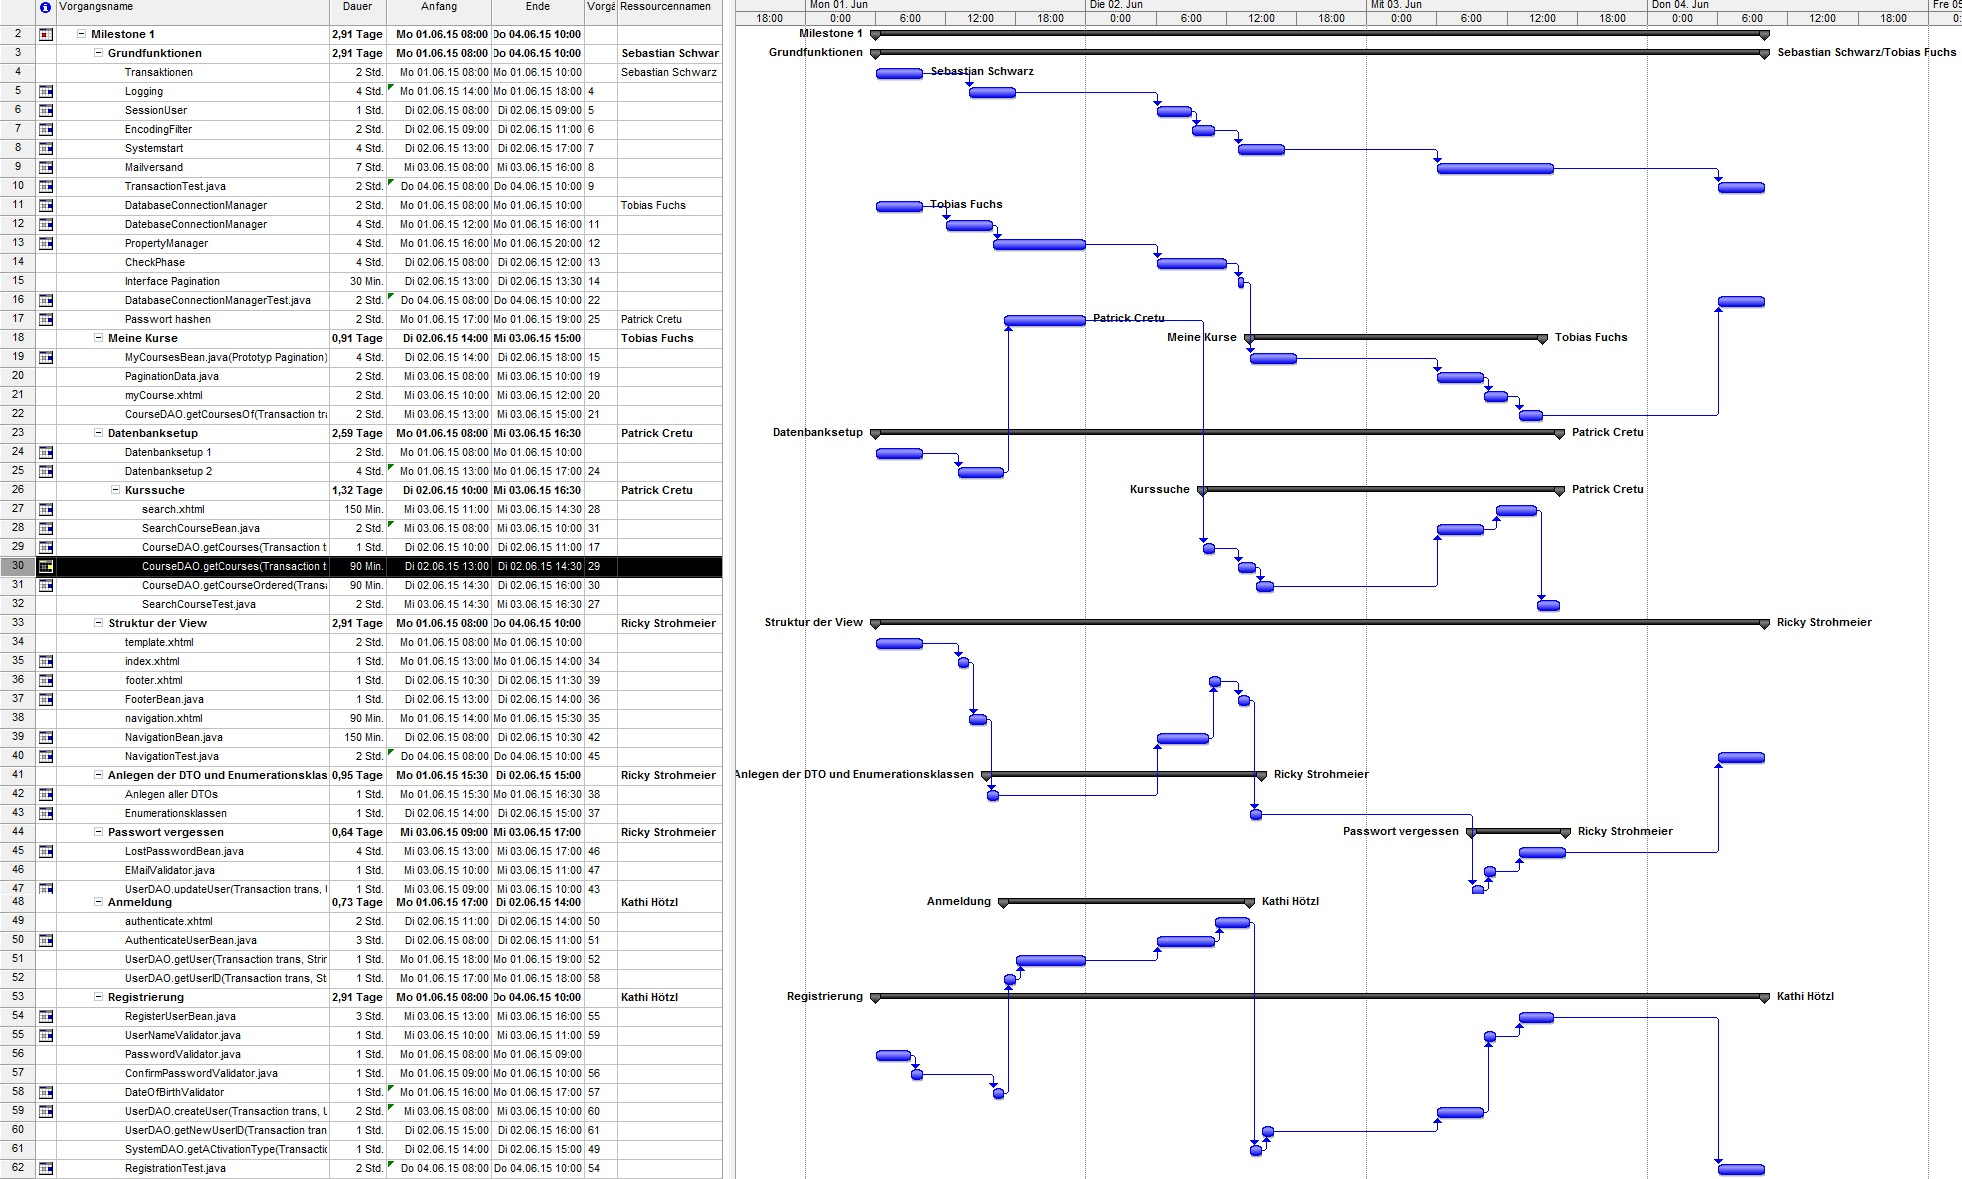
\includegraphics[width=0.8\linewidth, angle=90]{Grafiken/Milestone1Gantt}
 		\caption{GANTT-Diagramm Milestone 1}
 		\label{fig:GANTT-Diagramm Milestone 1}
 \end{figure}


\clearpage
\subsection{PERT-Diagramm Milestone 1}
\begin{figure}[h]
	\centering
	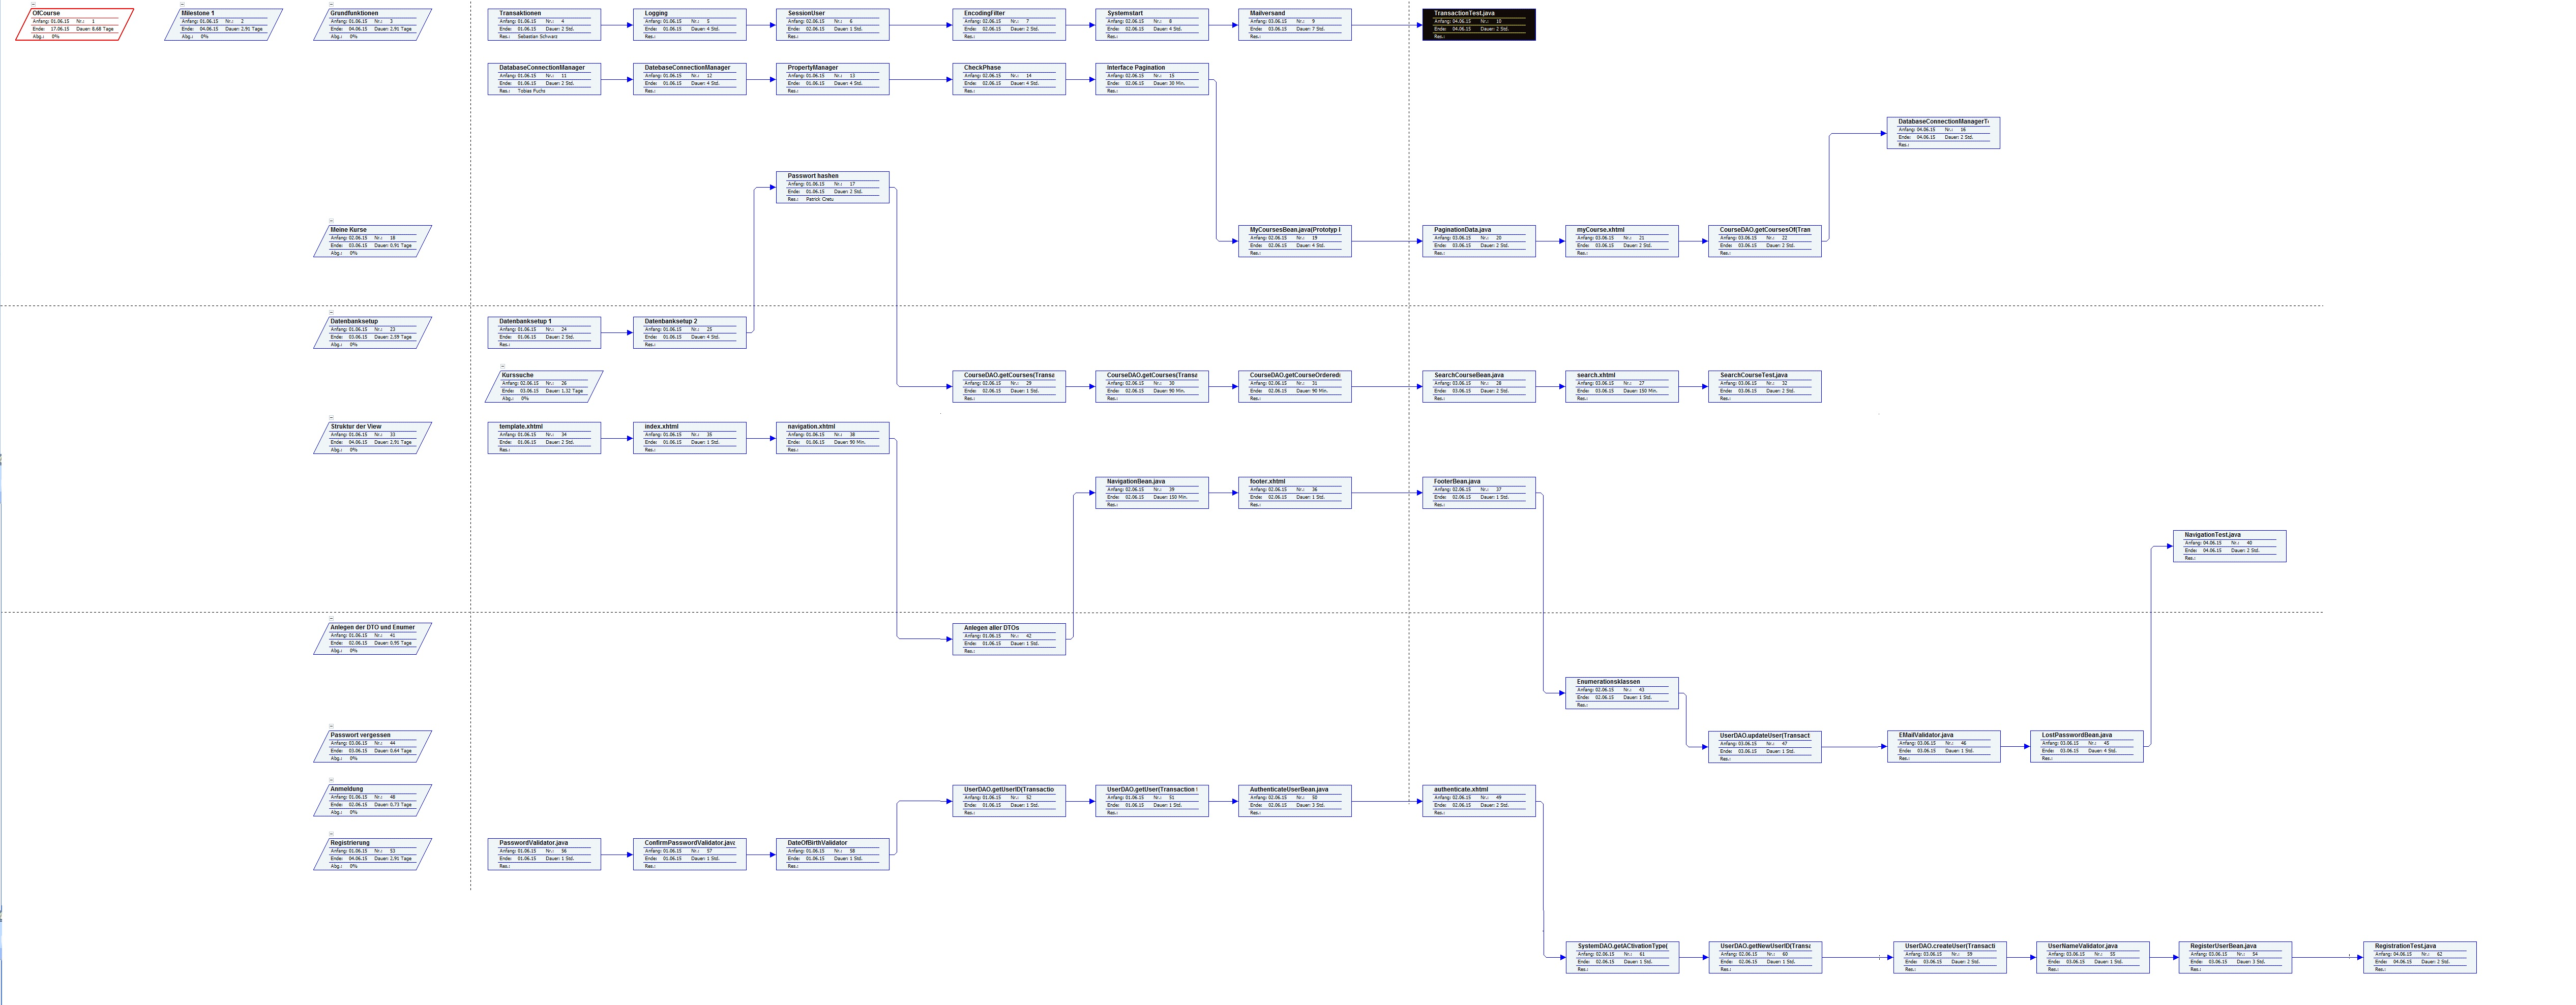
\includegraphics[width=1.0\linewidth, angle=90]{Grafiken/Milestone1Pert}
	\caption{PERT-Diagramm Milestone 1}
	\label{fig:PERT-Diagramm Milestone 1}
\end{figure}
\clearpage
\section{Milestone 2}
\subsection{GANTT-Diagramm Milestone 2}
\begin{figure}[h]
	\centering
	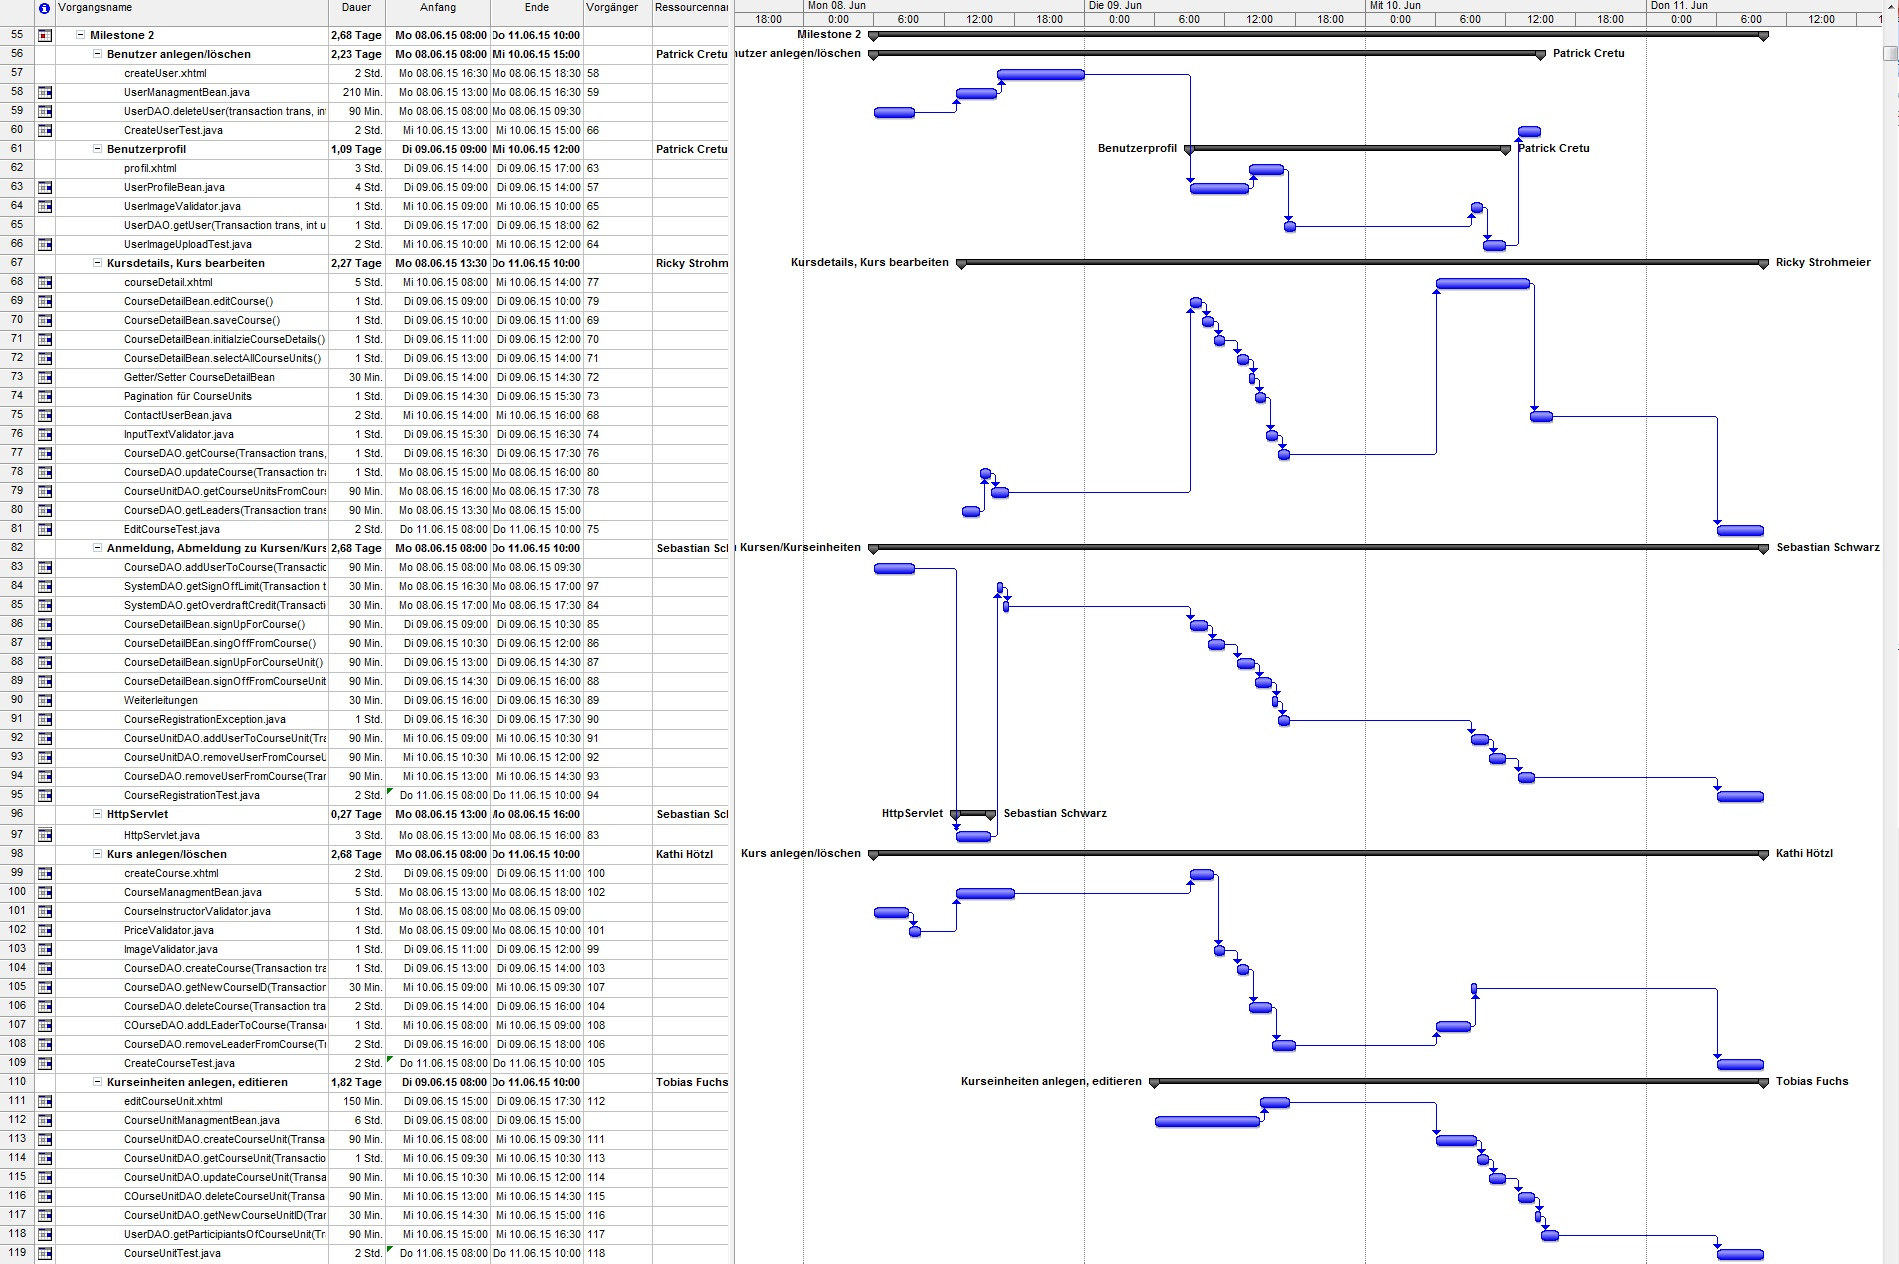
\includegraphics[width=1.0\linewidth, angle=90]{Grafiken/Milestone2Gantt}
	\caption{GANTT-Diagramm Milestone 2}
	\label{fig:GANTT-Diagramm Milestone 2}
\end{figure}

\clearpage
\subsection{PERT-Diagramm Milestone 2}
\begin{figure}[h]
	\centering
	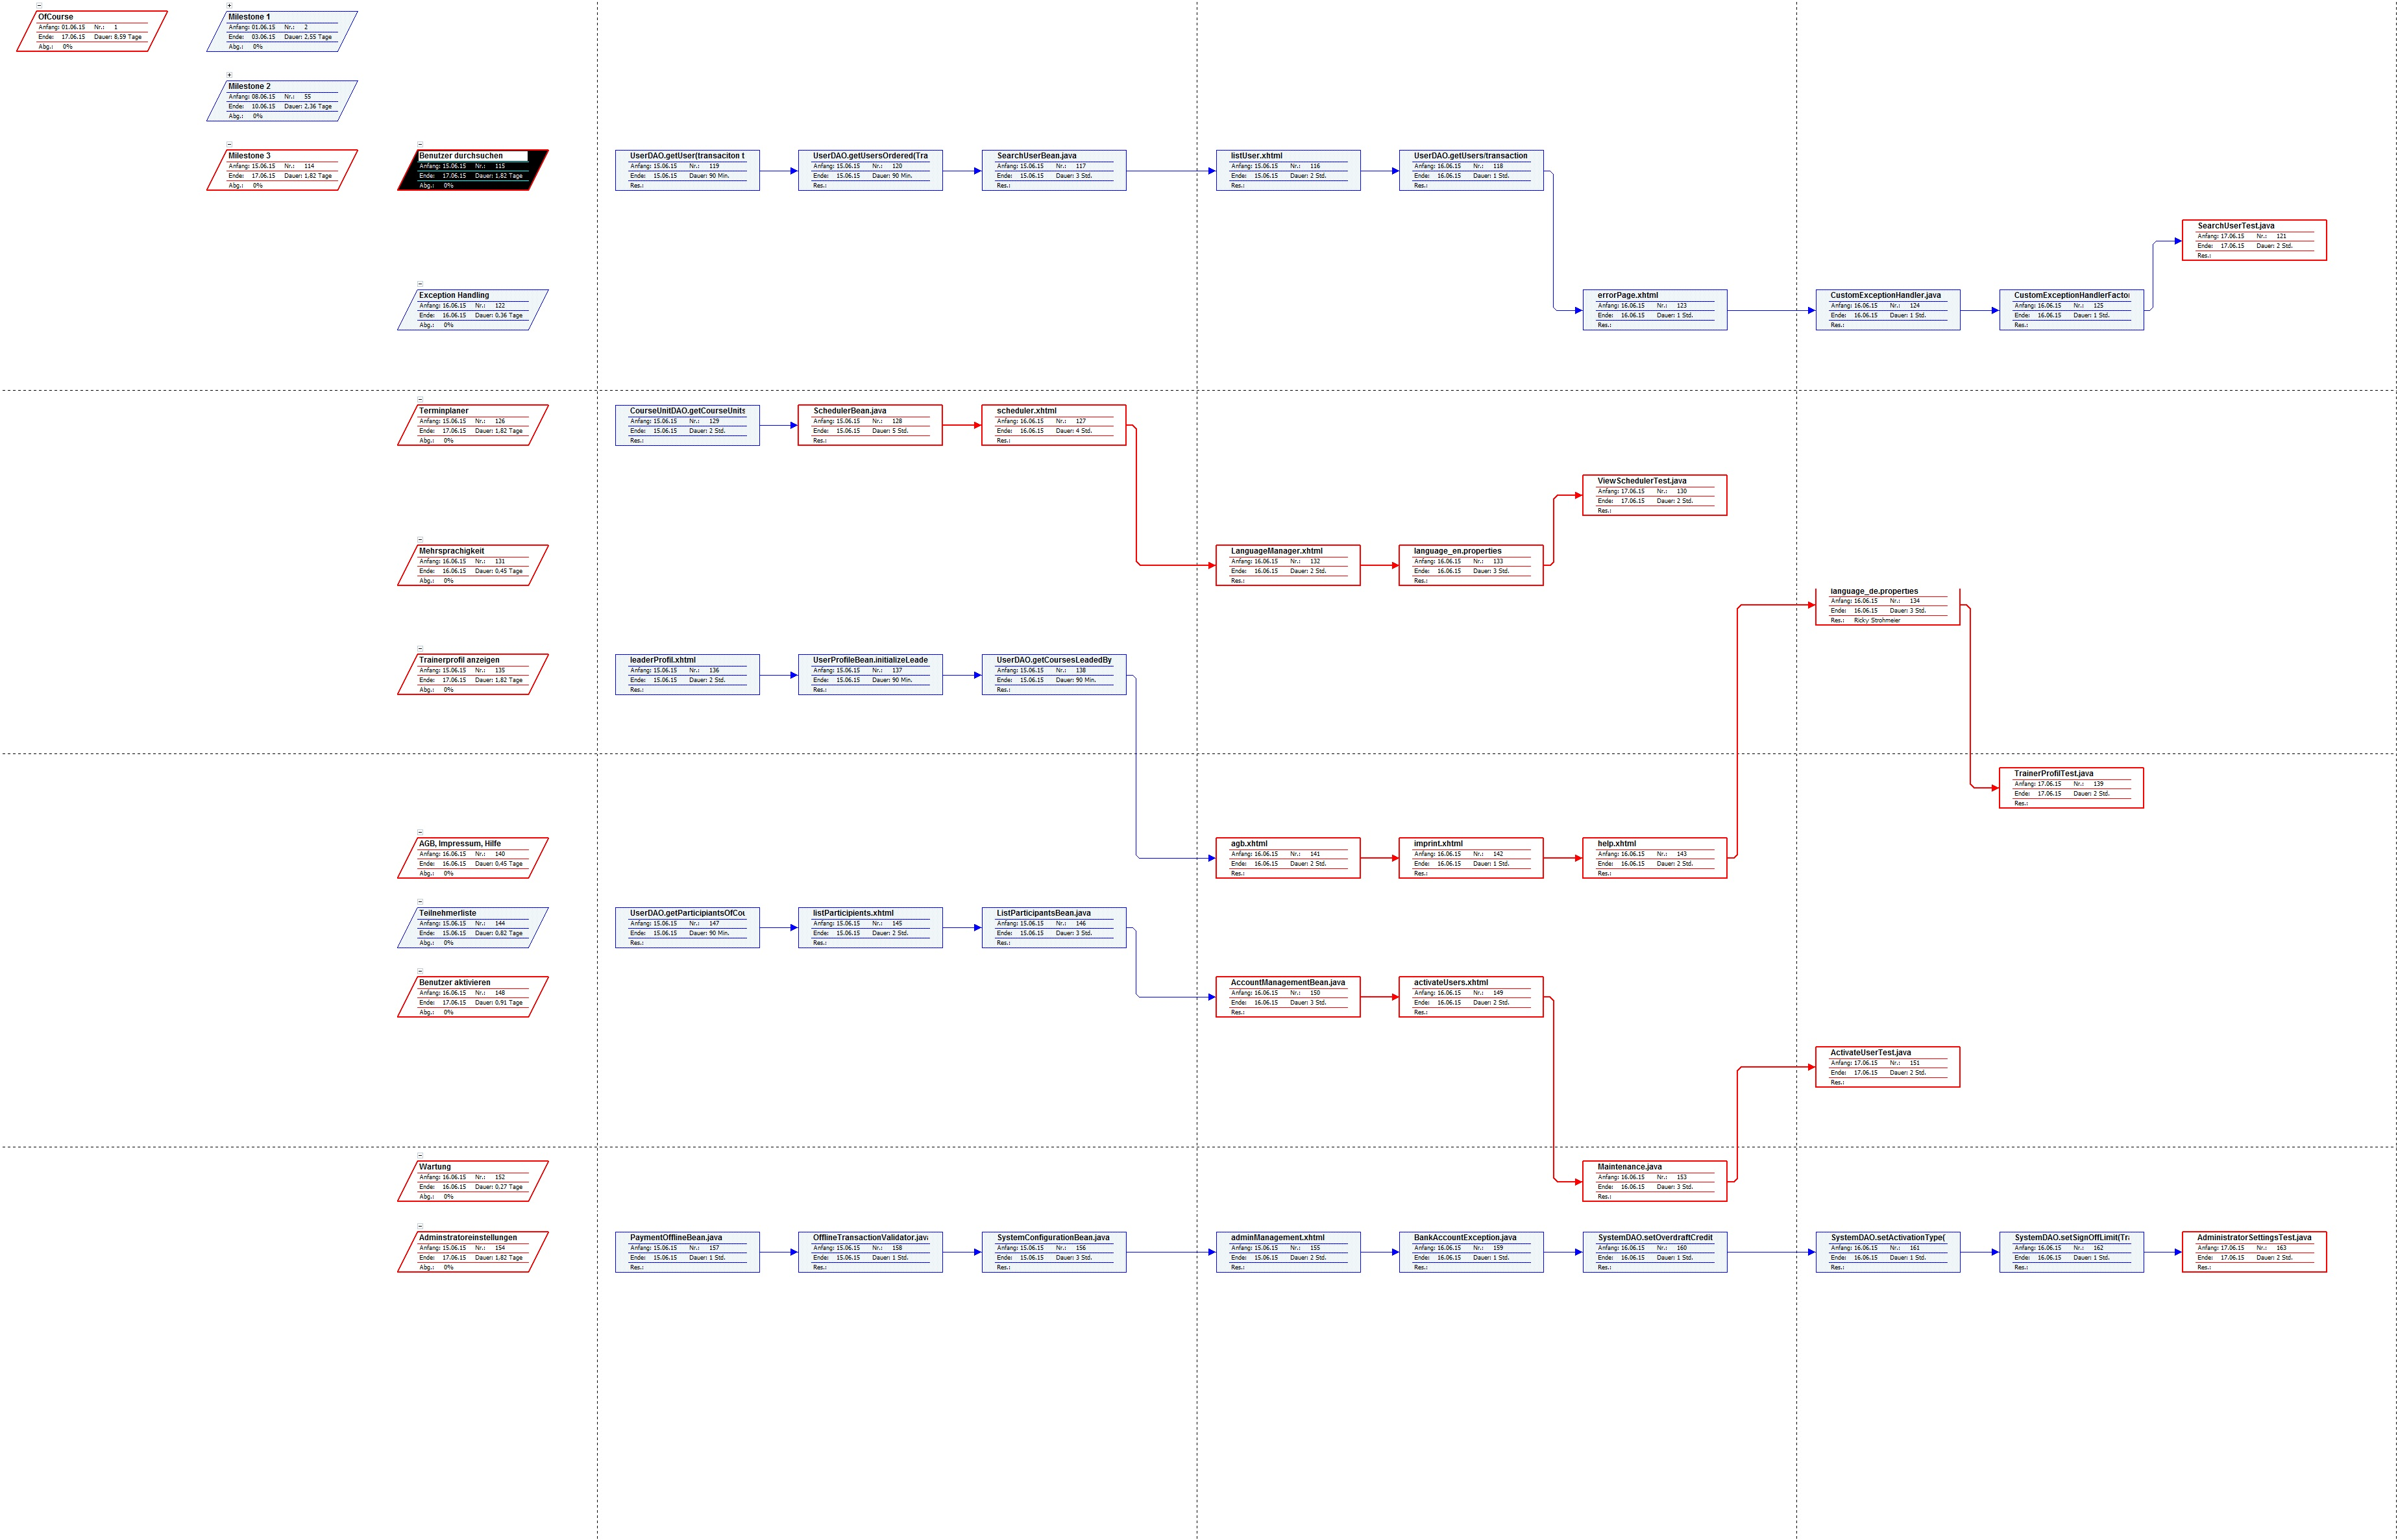
\includegraphics[width=1.0\linewidth, angle=90]{Grafiken/Milestone2Pert}
	\caption{PERT-Diagramm Milestone 2}
	\label{fig:PERT-Diagramm Milestone 2}
\end{figure}
\clearpage

\section{Milestone 3}
\subsection{GANTT-Diagramm Milestone 3}
\begin{figure}[h]
	\centering
	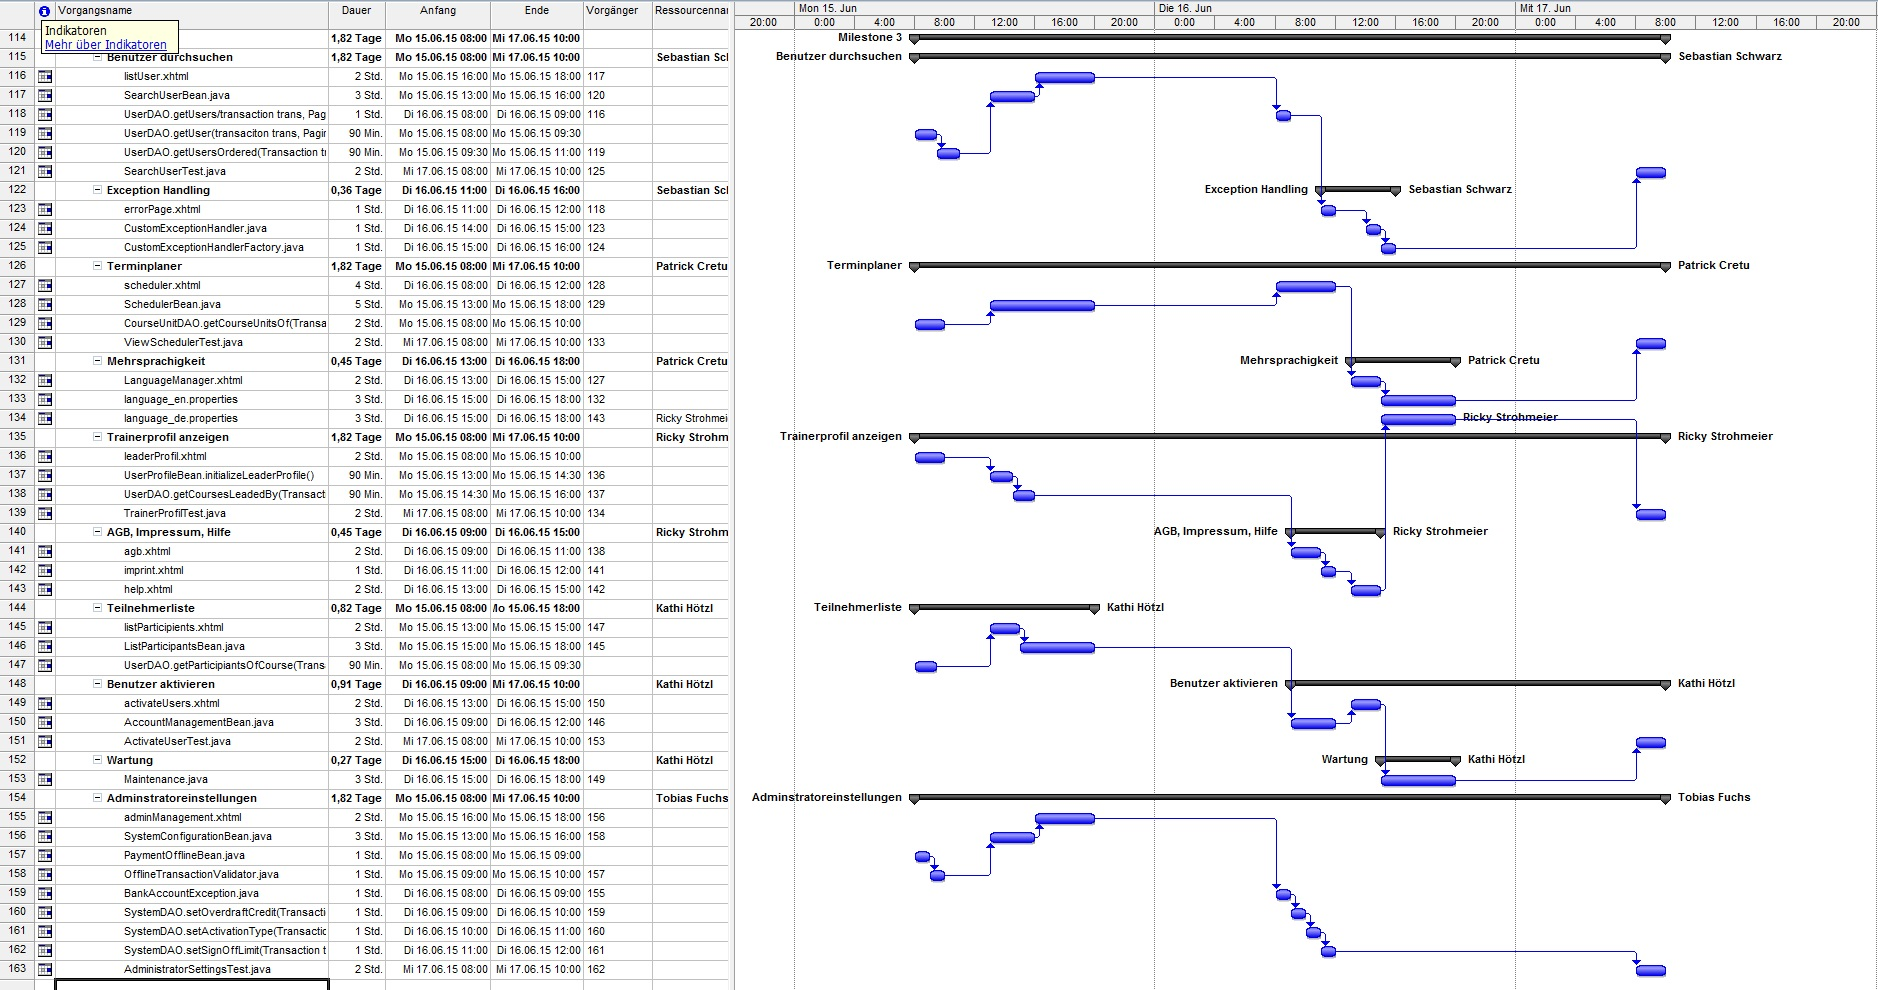
\includegraphics[width=1.0\linewidth, angle=90]{Grafiken/Milestone3Gantt}
	\caption{GANTT-Diagramm Milestone 3}
	\label{fig:GANTT-Diagramm Milestone 3}
\end{figure}
\clearpage

\subsection{PERT-Diagramm Milestone 3}
\begin{figure}[h]
	\centering
	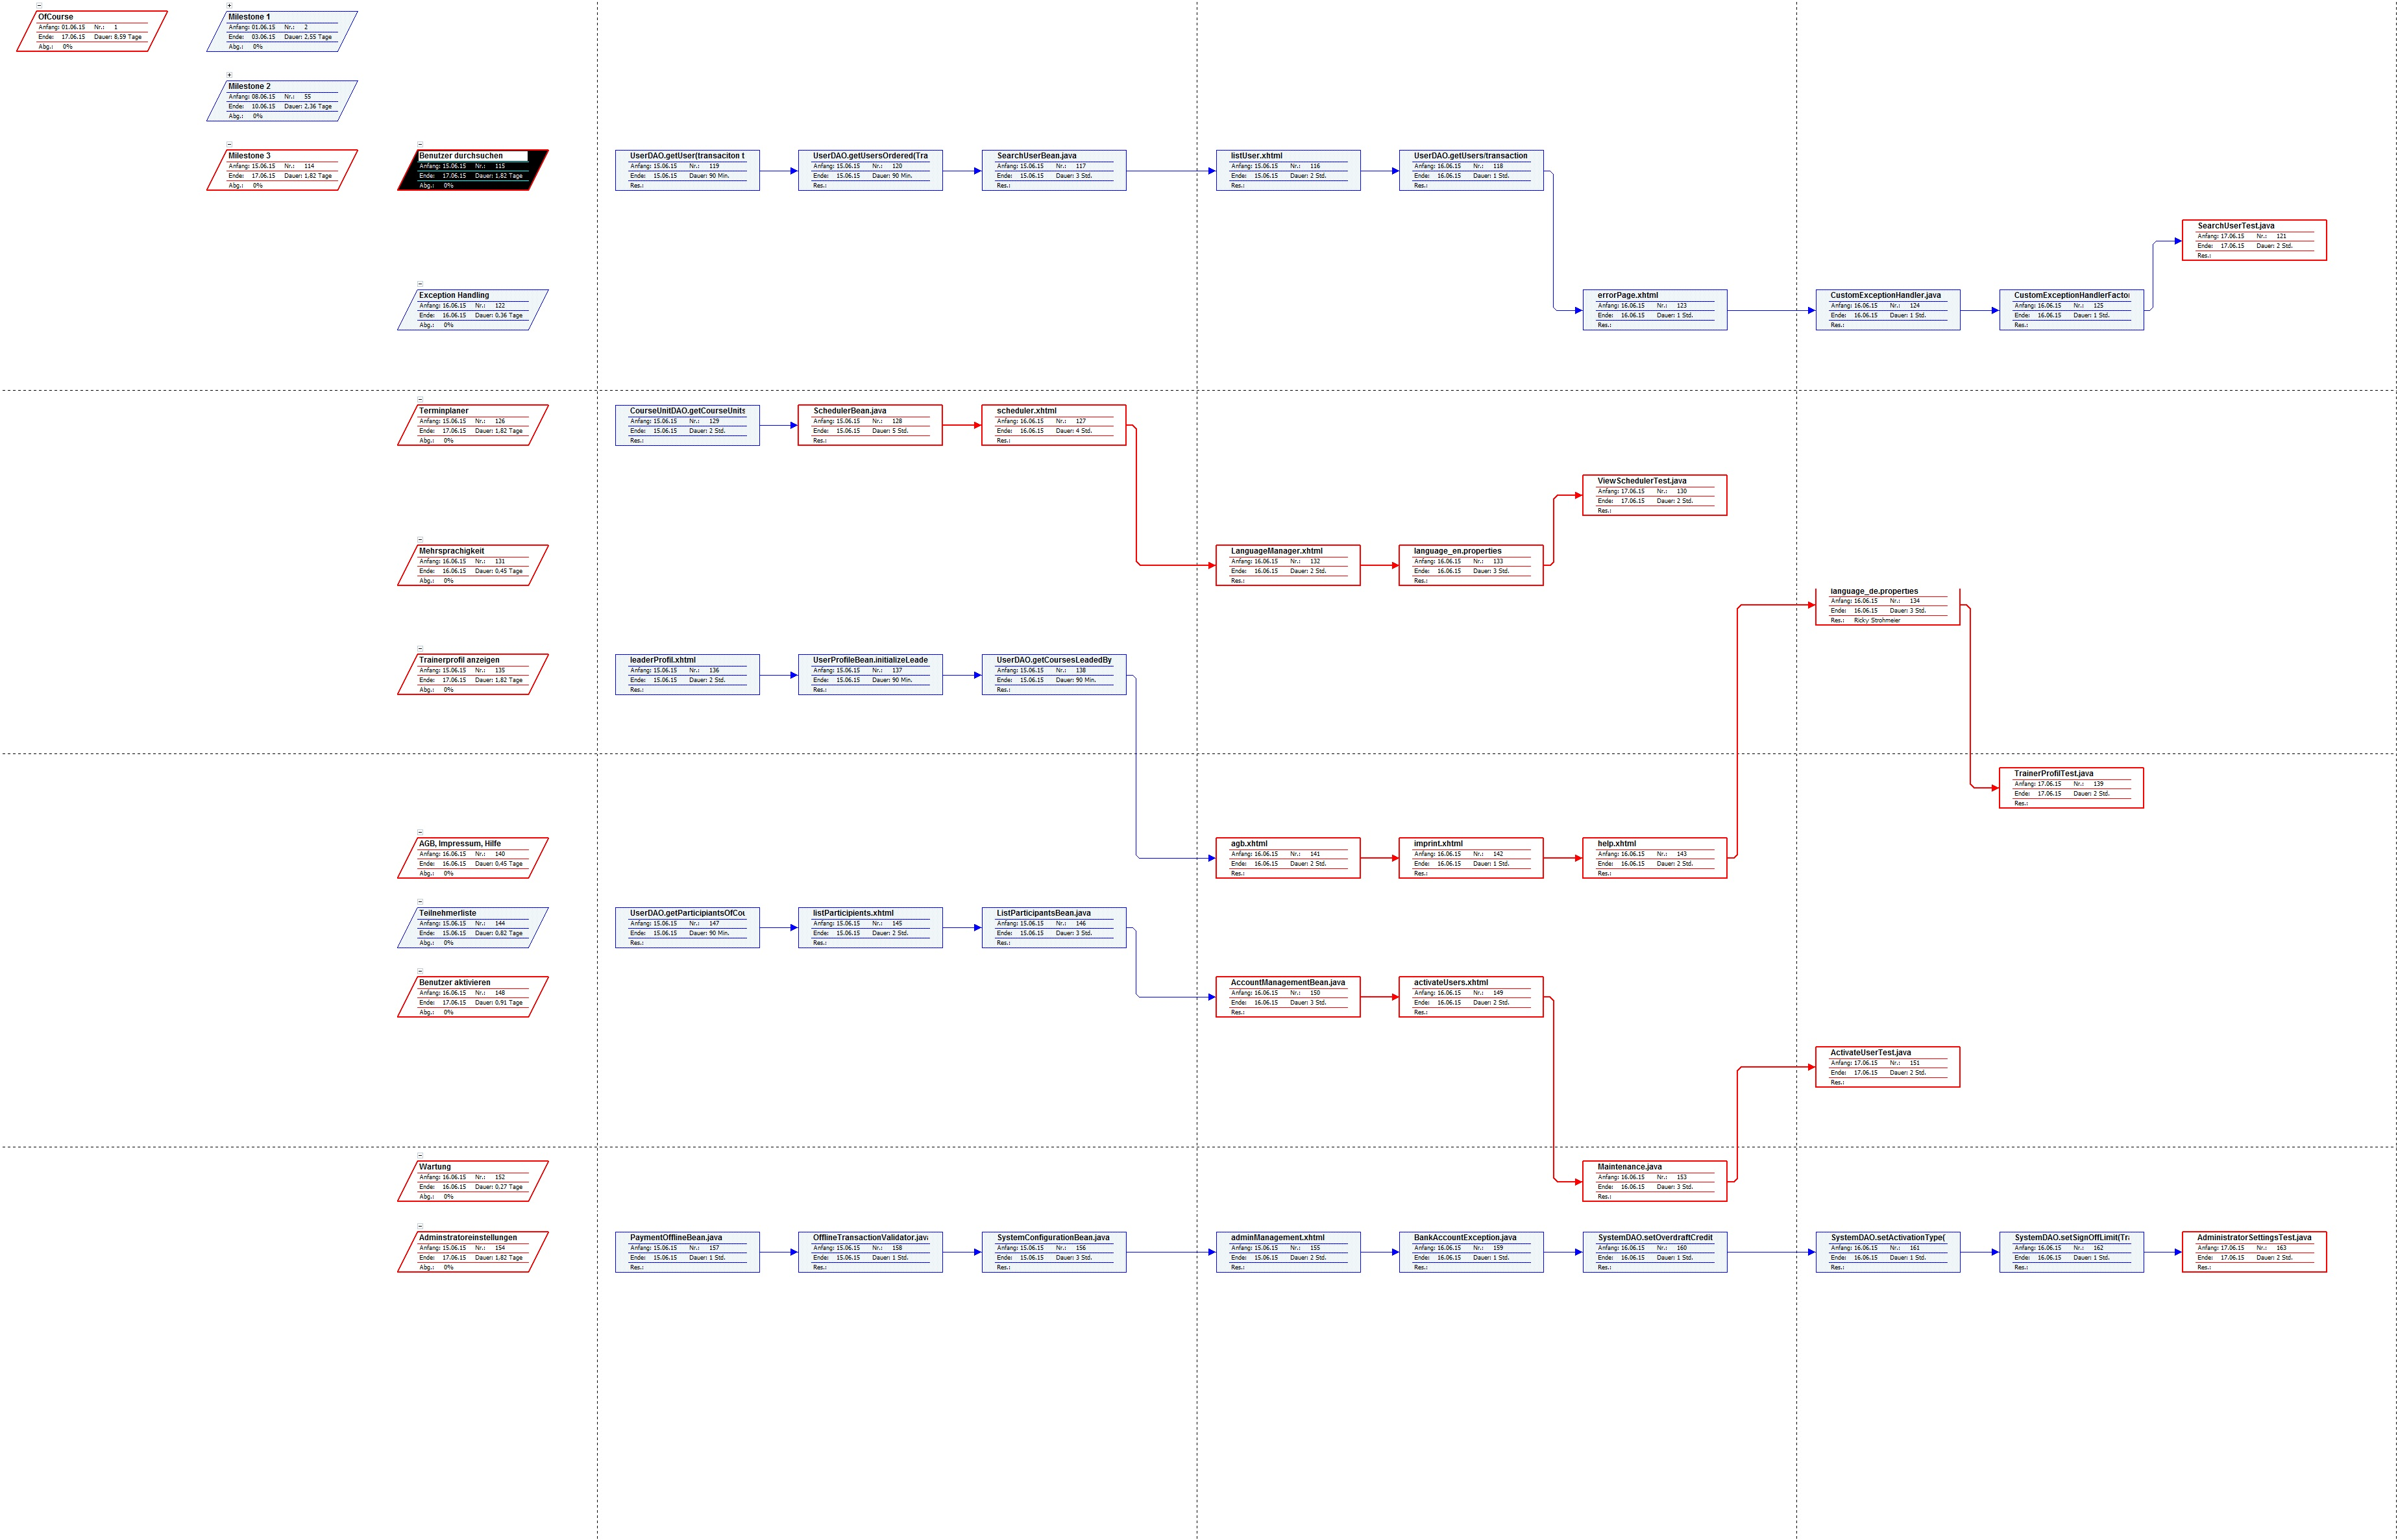
\includegraphics[width=1.0\linewidth, angle=90]{Grafiken/Milestone3PERT}
	\caption{PERT-Diagramm Milestone 3}
	\label{fig:PERT-Diagramm Milestone 3}
\end{figure}
\clearpage
\chapter{Expertenliste}

In diesem Kapitel werden die Spezialgebiete der jeweiligen Gruppenmitglieder aufgelistet(vgl. Tabelle \ref{fig:spezialgebiete}).
In der Planung ist darauf geachtet worden, dass der jeweilige Spezialist auch den Code, der sein
Spezialgebiet betrifft, implementiert.
Sofern dies nicht möglich ist, sind die Spezialisten trotzdem stets Ansprechpartner auf
den genannten Gebieten.\ \\
\ \\
\begin{table}[h]
	\begin{center}
	\begin{tabular}{|p{6cm}|p{6cm}|}
		\hline \textbf{Name} & \textbf{Spezialgebiet}  \\ 
		\hline Katharina Hölzl & LaTeX \newline
		                         GitHub \newline
		                         Tests    \\ 
		\hline Ricky Strohmeier & Bootstrap \newline
		                          Facelets \newline
		                          DTO  \\ 
		\hline Sebastian Schwarz & Transaktionsmanagement \newline
		                           Java Mail API \newline
		                           Konfigurationsadateien \\ 
		\hline Tobias Fuchs &    DatabaseConenctionManager \newline
		                         Pagination \newline
		                         Phase Listener \newline
		                         UML \\ 
		\hline Patrick Cretu &  SQL \newline
		                        Fileupload \newline
		                        Mehrsprachigkeit \newline
		                        ER - Diagramm \newline
		                        DAO\\ 
		\hline 
	\end{tabular} 
\caption{Spezialgebiete}
\label{fig:spezialgebiete}
\end{center}
\end{table}

\end{document}